% Szglab4
% ===========================================================================
%
%
% Szglab4
% ===========================================================================
%
\documentclass[11pt,oneside]{scrbook}

\usepackage[utf8]{inputenc}
\usepackage[T1]{fontenc}

\usepackage{fancyhdr}

\usepackage[magyar]{babel}

\usepackage{longtable}

\usepackage[usenames]{color}

\usepackage{float}

\usepackage{times}

\usepackage{listings}

\usepackage{graphicx}

\usepackage{epstopdf}

\usepackage{includes/szglab4}

\usepackage[%
	pdftitle={Szglab 4},% A PDF dokumentum címe.
	pdfauthor={such\_team},% Szerző(k) neve(i)
	pdfsubject={Szglab 4},% A PDF dokumentum témája
	pdfcreator={MiKTeX, LaTeX with hyperref and KOMA-Script}, % A PDF dokumentum készült ...
	pdfkeywords={Szglab4},% Kulcsszavak
	pdfpagemode=UseOutlines,% Tartalomjegyzék megjelenítése megnyitáskor
	pdfdisplaydoctitle=true,% Fájlnév helyett a dokumentum neve jelenjen meg
	pdflang=hu,% A dokumentum nyelve
	unicode
]{hyperref}

\definecolor{LinkColor}{rgb}{0,0,0}
\definecolor{ListingBackground}{rgb}{1,1,1}

\hypersetup{%
	colorlinks=true,% Színes linkek aktiválása a dokumentumban (keretek nélkül)
	linkcolor=LinkColor,%    szín beállítása
	citecolor=LinkColor,%    szín beállítása
	filecolor=LinkColor,%    szín beállítása
	menucolor=LinkColor,%    szín beállítása
	urlcolor=LinkColor,%     URL hivatkozások színe
	bookmarksnumbered=true
}

\newenvironment{nopb}
  {\par\nobreak\vfil\penalty0\vfilneg
   \vtop\bgroup}
  {\par\xdef\tpd{\the\prevdepth}\egroup
   \prevdepth=\tpd}

%
% ===========================================================================
% EOF
%

%
\csapat{\team}{27}
\konzulens{Szabó Ádám Imre}

\newcommand{\adam}[0]{Nusser Ádám}
\newcommand{\antal}[0]{Szabó Antal}
\newcommand{\bator}[0]{Tallér Bátor}
\newcommand{\torok}[0]{Török Attila}

\newcommand{\vadam}[0]{Nusser}
\newcommand{\vantal}[0]{Szabó}
\newcommand{\vbator}[0]{Tallér}
\newcommand{\vtorok}[0]{Török}

\taga{\adam}{P7PY3B}{nusee0726@hotmail.com}
\tagb{\antal}{R75PCE}{szabo.antal.92@gmail.com}
\tagc{\bator}{UGA4OQ}{tallerbator@gmail.com}
\tagd{\torok}{FULGDF}{torokati44@gmail.com}
\datum{\today}
%
\begin{document}
%
% Nem aktuális sorokat kommentezni
%\fedlap{Szoftver labor 4. házi feladat}
%\fedlap{2. Követelmény, projekt, funkcionalitás}
%\fedlap{3. Analízis modell kidolgozása 1}
%\fedlap{4. Analízis modell kidolgozása 2}
%\fedlap{5. Szkeleton tervezése}
%\fedlap{6. Szkeleton beadás}
%\fedlap{7. Prototípus koncepciója}
%\fedlap{10. Prototípus beadás}
%\fedlap{11. Grafikus felület specifikációja}
\fedlap{13. Grafikus változat beadása}
%
% Tartalomjegyzék és ábrák jegyzéke
%
\clearpage \tableofcontents \pagestyle{fancy}
\clearpage \listoffigures \pagestyle{fancy}
%
% Nem aktuális fejezetek kikommentezve
%
%\setcounter{chapter}{1}
%% Szglab4
% ===========================================================================
%

\chapter{Követelmény, projekt, funkcionalitás}

\thispagestyle{fancy}

\section{Bevezetés}

\subsection{Cél}

\comment{A dokumentum célja.}

\subsection{Szakterület}

\comment{A kialakítandó szoftver milyen területen használható, milyen célra.}

\subsection{Definíciók, rövidítések}
\comment{A dokumentumban használt definíciók, rövidítések magyarázata.}

\subsection{Hivatkozások}
\comment{A dokumentumban használt anyagok, web-oldalak felsorolása}

\subsection{Összefoglalás}
\comment{A dokumentum további részeinek rövid ismertetése}

\section{Áttekintés}
\subsection{Általános áttekintés}
\comment{A kialakítandó szoftver legmagasabb szintű architekturális képe. A fontosabb alrendszerek felsorolása, a közöttük kialakítandó interfészek lényege, a felhasználói kapcsolatok alapja. Esetleges hálózati és adattárolási elvárások.}

\subsection{Funkciók}
\comment{A feladat kb. 4000 karakteres (kb 1,5 oldal) részletezettségű magyar nyelvű leírása. Nem szerepelhetnek informatikai kifejezések.}

\subsection{Felhasználók}
\comment{A felhasználók jellemzői, tulajdonságai}

\subsection{Korlátozások}
\comment{Az elkészítendő szoftverre vonatkozó – általában nem funkcionális - előírások, korlátozások.}

\subsection{Feltételezések, kapcsolatok}
\comment{A dokumentumban használt anyagok, web-oldalak felsorolása}

\section{Követelmények}
\subsection{Funkcionális követelmények}


\comment{Az alábbi táblázat kitöltésével készítendő. Dolgozzon ki követelmény azonosító rendszert! Az ellenőrzés módja szokásosan bemutatás és/vagy kiértékelés. Prioritás lehet alapvető, fontos, opcionális. Az alapvető követelmények nem teljesítése végzetes. Forrás alatt a követelményt előíró anyagot, szervezetet kell érteni. Esetünkben forrás lehet maga a csapat is, mikor ő talál ki követelményt. Use-case-ek alatt az adott követelményt megvalósító használati esete(ke)t kell megadni.}

% Azonosító, Leírás, Ellenőrzés, Prioritás, Forrás, Use-case, Komment
\begin{longtable}{| l | l | l | l | l | l | l |}
\hline
\textbf{Azonosító}   & \textbf{Leírás} & \textbf{Ellenőrzés} & \textbf{Prioritás} & \textbf{Forrás} & \textbf{Use-case} & \textbf{Komment} \tabularnewline
\hline\hline
... & ... & ... & ... & ... & ... & ... \tabularnewline
\hline
\end{longtable}

\subsection{Erőforrásokkal kapcsolatos követelmények}

\comment{A szoftver fejlesztésével és használatával kapcsolatos számítógépes, hardveres, alapszoftveres és egyéb architekturális és logisztikai követelmények}

% Azonosító, Leírás, Ellenőrzés, Prioritás, Forrás, Komment
\begin{longtable}{| l | l | l | l | l | l |}
\hline
\textbf{Azonosító}   & \textbf{Leírás} & \textbf{Ellenőrzés} & \textbf{Prioritás} & \textbf{Forrás} & \textbf{Komment} \tabularnewline
\hline\hline
... & ... & ... & ... & ... & ... \tabularnewline
\hline
\end{longtable}


\subsection{Átadással kapcsolatos követelmények}
\comment{A szoftver átadásával, telepítésével, üzembe helyezésével kapcsolatos követelmények}

% Azonosító, Leírás, Ellenőrzés, Prioritás, Forrás, Komment
\begin{longtable}{| l | l | l | l | l | l |}
\hline
\textbf{Azonosító}   & \textbf{Leírás} & \textbf{Ellenőrzés} & \textbf{Prioritás} & \textbf{Forrás} & \textbf{Komment} \tabularnewline
\hline\hline
... & ... & ... & ... & ... & ... \tabularnewline
\hline
\end{longtable}

\subsection{Egyéb nem funkcionális követelmények}
\comment{A biztonsággal, hordozhatósággal, megbízhatósággal, tesztelhetőséggel, a felhasználóval kapcsolatos követelmények}

% Azonosító, Leírás, Ellenőrzés, Prioritás, Forrás, Komment
\begin{longtable}{| l | l | l | l | l | l |}
\hline
\textbf{Azonosító}   & \textbf{Leírás} & \textbf{Ellenőrzés} & \textbf{Prioritás} & \textbf{Forrás} & \textbf{Komment} \tabularnewline
\hline\hline
... & ... & ... & ... & ... & ... \tabularnewline
\hline
\end{longtable}


\section{Lényeges use-case-ek}
\comment{A 2.3.1-ben felsorolt követelmények közül az alapvető és fontos követelményekhez tartozó használati esetek megadása az alábbi táblázatos formában.}

\subsection{Use-case leírások}

\usecase
{Új játék indítása}
{Új játék indul el}
{Játékos}
{1. A játékos kiválasztja a menüben az "Új játék" feliratú gombot, és megnyomja. \newline
2. Ezután kiválaszthatja  a nehézséget és a pályát. \newline
3. Elindul a játék a kiválasztott pályával és nehézséggel.}

\usecase
{Pálya kiválasztása}
{Ki kell választani a pályát amelyen játszani kíván.}
{Játékos}
{Új játék indítása után egy listából ki kell választani a pályát amelyen játszani kíván.}

\usecase
{Nehézségi szint kiválasztása}
{Ki kell választani, hogy milyen nehézségen kíván játszani.}
{Játékos}
{Új játék indítása, és a pálya kiválasztása után, ki kell választani három opció közül,
 hogy mennyire legyen a játék nehéz.}

\usecase
{Torony építése}
{Új tornyot épít}
{Játékos}
{Olyan mezőre kattintva, ahol nincsen út vagy torony, ott új torony épül, 
ha van elég varázserő hozzá.}

\usecase
{Akadály építése}
{Új akadályt épít}
{Játékos}
{Olyan mezőre kattintva ahol út van, és még nincsen akadály, ott akadály épül,
ha van elég varázserő hozzá.}

\usecase
{Torony/akadály enchant-olás}
{Már létező tornyot vagy akadályt enchant-olunk}
{Játékos}
{Toronyra vagy akadályra kattintva ki kell választani, hogy milyen drágakővel szeretné enchant-olni, 
és ha van elég varázserő hozzá akkor megtörténik az enchant.}

\usecase
{Feladás}
{Feladjuk a jelenlegi játékot}
{Játékos}
{A feladás gombra kattintva a játék végetér, és megnyílik a főmenü.}

\usecase
{Kilépés}
{Kilép az alkalmazásból}
{Játékos}
{Az ablak jobb felső sarkában, a bezárásra kattintva az alkalmazás kilép.}

\subsection{Use-case diagram}

\begin{figure}[ht!]
\centering
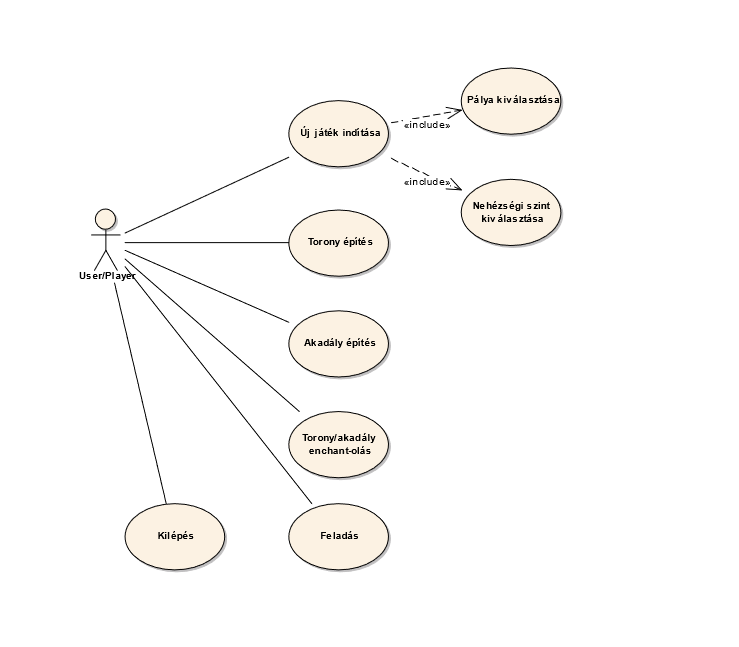
\includegraphics[width=170mm]{images/UseCase.png}
\caption{Use-case diagram}
\label{overflow}
\end{figure}

\section{Szótár}
\comment{A szótár a követelmények alapján készítendő fejezet. Egy szótári bejegyzés definiálásához csak más szótári bejegyzések és köznapi – a feladattól független – fogalmak használhatók fel. A szótár mérete kb. 1-2 oldal legyen.}

\section{Projekt terv}
\comment{Tartalmaznia kell a projekt végrehajtásának lépéseit, a lépések, eredmények határidejét, az egyes feladatok elvégzéséért felelős személyek nevét és beosztását, a szükséges erőforrásokat, stb. Meg kell adni a csoportmunkát támogató eszközöket, a választott technikákat! Definiálni kell, hogy hogyan történik a dokumentumok és a forráskód megosztása!}



%\pagebreak
%% Szglab4
% ===========================================================================
%
\section{Napló}

\begin{naplo}

\bejegyzes
{2014.02.19.~08:15~}
{1,5 óra}
{\vadam\newline
\vantal\newline
\vbator\newline
\vtorok}
{Kezdeti megbeszélés, use-case-ek átbeszélése, feladatok kiosztása}

\bejegyzes
{2014.02.21.~18:00~} % Kezdet
{1 óra} % Időtartam
{\vantal} % Résztvevők
{Dokumentáció elkezdése} % Leírás

\bejegyzes
{2014.02.22.~13:30~}
{3 óra}
{\vadam}
{Use-case -ek leírása, és diagram készítése.}

\bejegyzes
{2014.02.22.~18:00~}
{2 óra}
{\vbator}
{Követelmények befejezése}

\bejegyzes
{2014.02.22.~19:00~}
{1 óra}
{\vadam}
{Use-case-ek befejezése}

\bejegyzes
{2014.02.22.~21:30~}
{1,5 óra}
{\vadam\newline
\vantal\newline
\vbator\newline
\vtorok}
{Közös megbeszélés}

\bejegyzes
{2014.02.23.~17:00~}
{2 óra}
{\vbator}
{Projekt terv elkészítése}

\bejegyzes
{2014.02.23.~18:00~}
{0,5 óra}
{\vantal}
{Bevezetés definíciók nélkül}

\bejegyzes
{2014.02.23.~21:30~}
{1,5 óra}
{\vantal}
{Definíciók}
=======
{\antal}
{Definíciók elkészítése}

\bejegyzes
{2014.02.24.~01:00~}
{1 óra}
{\vantal}
{Szótár elkészítése}

\end{naplo}

%%
%\setcounter{chapter}{2}
%% Szglab4
% ===========================================================================
%
\chapter{Analízis modell kidolgozása 1}

\thispagestyle{fancy}

\section{Objektum katalógus}

\comment{Minden, a feladatban szereplő objektum rövid, egy-két bekezdés hosszú ismertetése. Meg kell jelenjen minden objektumhoz, hogy mi a felelőssége. Informális leírás, ezért nem kell foglalkozni az örökléssel, az interfészekkel, az absztrakt osztályokkal, a segédosztályokkal.}

\subsection{Tower}
Egy tornyot valósít meg. Ha egy ellenség a hatókörébe ér, akkor elindít egy \textbf{Projectile}-t az irányába, a tüzelési gyakoriságának megfelelő időközönként. Ha több ellenfél van a hatókörében, akkor arra lő, aki a legközelebb van a célhoz.

\subsection{Obstacle}
Egy akadályt valósít meg. Ha egy ellenség belelép egy olyan mezőbe, amin van egy \textbf{Obstacle}, akkor azt egy bizonyos mértékben lelassítja, az ellenség fajától függően.

\subsection{Map}
A Map a pályát képviseli, melyben NxM darab cella van. A pálya egy külső fájlból betölthető, ami új játék indulásakor fog megtörténni, miután kiválasztja a játékos a pályát. A pálya különböző tulajdonságai is lekérdezhetőek, amelyek majd a kirajzoláshoz kellenek.

\subsection{Tile}
A Tile objektumból egy NxM -es tömböt fog tárolni a Map objektum. Ezek a pálya egyes celláit fogják képviselni. Egy cellán lehet maximum egy darab épület, amely vagy egy torony, vagy egy akadály, attól függően, hogy van-e a cellán út, vagy nincsen. A cellán levő épület referenciája lekérhető, vagy ha még nincsen rajta, és a cellára kattintás történik, akkor épül egy megfelelő épület.

Ha egy cellán van út, akkor lekérdezhető, hogy az a cella milyen távol van a céltól (az utat követve, cellákban mérve). Továbbá az is tárolva van, és lekérdezhető, hogy az út merre folytatódik (és az ellenségeknek merre kell majd menniük). Ha elágazás van, akkor véletlenszerűen választ irányt és arra küldi az ellenséget (ez minden egyes ellenségre véletlenszerű).

\subsection{Mission}
Egy Mission objektumban lesz eltárolva, hogy milyen ellenségek, mikor és honnan jönnek be a pályára. Ez a három adat majd egy segéd osztályban lesz összefogva, és egy tárolóban lesz tárolva. A játék főciklusa le tudja majd kérdezni a következő ellenséget, melyet az objektum visszaad, ha már elég idő eltelt az előző egység óta (ha nem akkor nem ad vissza egységet).

\subsection{Game}
Ez a játék logikáját magába foglaló osztály. Számon tartja a pályán lévő ellenfeleket, akadályokat és tornyokat, valamint végrehajtja a kiválasztott misszió által leírt forgatókönyvet, ami alapján az ellenségek érkeznek.

\subsection{EnemyType}
Leírja egy ellenségtípus (jelen esetben a négy faj: ember, tünde, törp vagy hobbit) tulajdonságait, mint például az alapsebessége és a kezdeti életereje. Minden ellenségnek van egy referenciája egy példányára, amely meghatározza a viselkedését.

\subsection{Enemy}
Az Enemy osztály példányai egy-egy ellenséget tárolnak. Rendelkeznek típussal (fajjal), pillanatnyi pozícióval, hátralévő életerővel. Az idő haladtával próbálnak végighaladni egy véletlenszerűen választott lehetséges útvonalon.

\subsection{Projectile}
Ez a class egy lövedék leírása. Amikor egy torony lő, akkor példányosítja ezt az osztályt a cél ellenség átadásával, így egy lövedék mindig a torony által meghatározott ellenség után megy, amit ha megfelelően megközelít (eltalálja az ellenséget), akkor levesz az életerejéből és megsemmisíti magát.

\subection{Gem}
Egy épületekre rakható varázskő tulajdonságait tárolja. A Game class fog példányokat létrehozni belőle, különböző tulajdonságokkal. Ha egy épületre rá van rakva egy fajta varázskő, akkor az épület egy referenciát tárol a példányára.


\section{Statikus struktúra diagramok}
\comment{Az előző alfejezet osztályainak kapcsolatait és publikus metódusait bemutató osztálydiagram(ok). Tipikus hibalehetőségek: csillag-topológia, szigetek.}

\begin{figure}[h]
\begin{center}
%\includegraphics[width=17cm]{chapters/chapter03/example.pdf}
\caption{x}
\label{fig:example1}
\end{center}
\end{figure}


\section{Osztályok leírása}
\comment{Az előző alfejezetben tárgyalt objektumok felelősségének formalizálása attribútumokká, metódusokká. Csak publikus metódusok szerepelhetnek. Ebben az alfejezetben megjelennek az interfészek, az öröklés, az absztrakt osztályok. Segédosztályokra még mindig nincs szükség. Az osztályok ABC sorrendben kövessék egymást. Interfészek esetén az Interfészek, Attribútumok pontok kimaradnak.}

\subsection{Building}
\begin{itemize}
\item Felelősség\\
%\comment{Mi az osztály felelőssége. Kb 1 bekezdés.} \\
Biztosít egy interfészt az épületek számára. Eltárolja az épülethez tartozó varázskövet.
\item Attribútumok
%\\\comment{Milyen attribútumai vannak}
	\begin{itemize}
		\item gem: eltárol egy referenciát egy \textbf{Gem} típusú objektumra, ami meghatározza, hogy az adott épület milyen echant alatt áll.
		\item int human: megadja mekkora a human típusú ellenfelekre kifejtett hatása az épületnek.
		\item int elf: megadja mekkora az elf típusú ellenfelekre kifejtett hatása az épületnek.
		\item int dwarf: megadja mekkora a dwarf típusú ellenfelekre kifejtett hatása az épületnek.
		\item int hobbit: megadja mekkora a hobbit típusú ellenfelekre kifejtett hatása az épületnek.
		\item \textbf{Tile} tile: egy referencia arra a mezőre, ahol az épület található.
	\end{itemize}
\item Metódusok\\
%\comment{Milyen publikus metódusokkal rendelkezik. Metódusonként egy-három mondat arról, hogy a metódus mit csinál.}
	\begin{itemize}
		\item \textbf{Gem} getGem(): visszaadja az épületen található varázskövet
		\item void setGem(\textbf{Gem} gem): beállítja az epületen lévő varázskövet. Ha már volt az épületen varázskő, akkor az előző megszűnik.
		\item void setTile(\textbf{Tile} tile)
		\item \textbf{Tile} getTile()
	\end{itemize}
\end{itemize}

\subsection{Tower}
\begin{itemize}
\item Felelősség\\
Felelős \textbf{Projectile}-ok létrehozásához, azok megfelelő felparaméterezésével. Továbbá felelős azért, hogy \textbf{Projectile}-okat csak a megadott időközönként lőjjön ki.
\item Attribútumok
	\begin{itemize}
		\item gem: eltárol egy referenciát egy \textbf{Gem} típusú objektumra, ami meghatározza, hogy az adott épület milyen echant alatt áll.
		\item Map<EnemyType, double>: megadja mekkora az adott típusú ellenfélre kifejtett hatása a toronynak
		\item \textbf{Tile} tile: egy referencia arra a mezőre, ahol az épület található.
	\end{itemize}
\item Metódusok
	\begin{itemize}
		\item \textbf{Projectile} attack(\textbf{Enemy} enemy): kilő egy \textbf{Projectile}-t a paraméterként megkapott ellenségre, majd a visszatérési értékében visszaadja azt. A \textbf{Projectile}-t felparaméterezi az ellenséghez megfelelő sebzési adatokkal.
		\item \textbf{Gem} getGem(): visszaadja az épületen található varázskövet
		\item void setGem(\textbf{Gem} gem): beállítja az epületen lévő varázskövet. Ha már volt az épületen varázskő, akkor az előző megszűnik.
		\item void setTile(\textbf{Tile} tile)
		\item \textbf{Tile} getTile()
	\end{itemize}
\end{itemize}

\subsection{Obstacle}
\begin{itemize}
\item Felelősség\\
Felelős \textbf{Projectile}-ok létrehozásához, azok megfelelő felparaméterezésével. Továbbá felelős azért, hogy \textbf{Projectile}-okat csak a megadott időközönként lőjjön ki.
\item Ősosztályok\\
\textbf{Building}
\item Attribútumok\\
		\item gem: eltárol egy referenciát egy \textbf{Gem} típusú objektumra, ami meghatározza, hogy az adott épület milyen echant alatt áll.
		\item Map<EnemyType, double>: megadja mekkora az adott típusú ellenfélre kifejtett hatása az akadálynak
		\item \textbf{Tile} tile: egy referencia arra a mezőre, ahol az épület található.
\item Metódusok
	\begin{itemize}
		\item double getSlowingFactor(\textbf{Enemy} enemy): visszatér azzal az értékkel, amivel az adott ellenfelet lassítja.
		\item \textbf{Gem} getGem(): visszaadja az épületen található varázskövet
		\item void setGem(\textbf{Gem} gem): beállítja az epületen lévő varázskövet. Ha már volt az épületen varázskő, akkor az előző megszűnik.
		\item void setTile(\textbf{Tile} tile)
		\item \textbf{Tile} getTile()
	\end{itemize}
\end{itemize}

\subsection{Map}
\begin{itemize}
\item Felelősség\\
%\comment{Mi az osztály felelőssége. Kb 1 bekezdés.}
Tartlamaz az összes cellára referenciát, felelős a kapott fájlból beolvasni a pályát, és felépíteni azt.
\item Ősosztályok\\
%\comment{Mely osztályokból származik (öröklési hierarchia)\newline
%Legősebb osztály $\rightarrow$ Ősosztály2 $\rightarrow$ Ősosztály3...}
-
\item Interfészek\\
%\comment{Mely interfészeket valósítja meg.}
-
\item Attribútumok\\
%\comment{Milyen attribútumai vannak}
	\begin{itemize}
		\item Tile[][]: A pályán található cellák tömbje, a pálya kirajzolásához használható.
	\end{itemize}
\item Metódusok\\
%\comment{Milyen publikus metódusokkal rendelkezik. Metódusonként egy-három mondat arról, hogy a metódus mit csinál.}
	\begin{itemize}
		\item Tile getTileAt(Vector position): Visszaadja a position helyen talalható cellát.
		\item void readMapFile(String file): Betölti a kapott elérési útvonalon a fájlt, és felépíti az alapján a pályát.
	\end{itemize}
\end{itemize}


\subsection{Mission}
\begin{itemize}
\item Felelősség\\
%\comment{Mi az osztály felelőssége. Kb 1 bekezdés.}
Felelőssége, felépíteni a listát, amely a beérkező ellenségeket és időzítésüket tartalmazza. Majd a megfelelő időközönként ki kell adja ezeket az egységeket a Game osztálynak.
\item Ősosztályok\\
%\comment{Mely osztályokból származik (öröklési hierarchia)\newline
%Legősebb osztály $\rightarrow$ Ősosztály2 $\rightarrow$ Ősosztály3...}
-
\item Interfészek\\
%\comment{Mely interfészeket valósítja meg.}
-
\item Attribútumok\\
%\comment{Milyen attribútumai vannak}
	\begin{itemize}
		\item List<Spawn> spawnList: a Spawn segédosztályban tárolt ellenség-idő-belépési pont, adatokat tárolja.
		\item int counter: méri az előző ellenség megjelenése óta eltelt ciklusokat.
	\end{itemize}
\item Metódusok\\
%\comment{Milyen publikus metódusokkal rendelkezik. Metódusonként egy-három mondat arról, hogy a metódus mit csinál.}
	\begin{itemize}
		\item Enemy getNextEnemy(): a spawnList listaból a következő elemet megvizsgaálja, és ha elegendő ciklus eltelt az előző ellenség megjelenése óta, akkor visszatér a kivett Spawn ellenségével.
		\item void readMissionFile(String file): Betölti a kapott elérési útvonalon a fájlt, és felépíti az alapján a listát (spawnList).
	\end{itemize}
\end{itemize}


\subsection{Tile}
\begin{itemize}
\item Felelősség\\
%\comment{Mi az osztály felelőssége. Kb 1 bekezdés.}
Egy cellán lehet maximum egy darab épület, amely vagy egy torony, vagy egy akadály, attól függően, hogy van-e a cellán út, vagy nincsen. A cellán levő épület referenciája lekérhető, vagy ha még nincsen rajta, és a cellára kattintás történik, akkor épül egy megfelelő épület. Felelős még az egyes ellenségek következő irányának a meghatározására, és vissza kell tudnia adni, hogy van-e rajta út, valamint ha van akkor milyen távol van a céltól.
\item Ősosztályok\\
%\comment{Mely osztályokból származik (öröklési hierarchia)\newline
%Legősebb osztály $\rightarrow$ Ősosztály2 $\rightarrow$ Ősosztály3...}
-
\item Interfészek\\
%\comment{Mely interfészeket valósítja meg.}
-
\item Attribútumok\\
%\comment{Milyen attribútumai vannak}
	\begin{itemize}
		\item Building building: a cellában levő epület.
		\item int distance: hányadik cella az utat követve a céltól.
		\item bool road: van-e út a cellában.
		\item double up: annak a valószinűsége, hogy a cellából felfelé fog menni az ellenség.
		\item double down: annak a valószinűsége, hogy a cellából lefelé fog menni az ellenség.
		\item double left: annak a valószinűsége, hogy a cellából balra fog menni az ellenség.
		\item double right: annak a valószinűsége, hogy a cellából jobbra fog menni az ellenség.
	\end{itemize}
\item Metódusok\\
%\comment{Milyen publikus metódusokkal rendelkezik. Metódusonként egy-három mondat arról, hogy a metódus mit csinál.}
	\begin{itemize}
		\item void buildTower(): a cellán egy tornyot épít.
		\item void buildObstacle(): a cellán egy akadályt épít.
		\item int getDistance(): vissza adja a distance értékét.
		\item bool isRoad(): vissza adja a road értékét.
		\item direction nextDirection(): visszad egy irány enum-ot, amely megadja az ellenség irányát.
		\item getBuilding(): visszatér a building referenciájával.
	\end{itemize}
\end{itemize}

\subsection{Game}
\begin{itemize}
\item Felelősség\\
A többi osztály nyilván tartása és összekötése, a játékbeli események vezérlése. A felhasználói felülettől érkező parancsok végrehajtása, és a játék állapotának rendelkezésre bocsájtása a kijelzéshez.

\item Attribútumok\\
%\comment{Milyen attribútumai vannak}
	\begin{itemize}
		\item ArrayList<Projectile> projectiles: Eltárolja a jelenleg játékban lévő lövedékeket.
		\item Map map: Referencia a kiválasztott pályára, amin a játék folyik.
		\item Mission mission: Referencia a kiválasztott misszióra, amely alapján zajlik a játék.
		\item ArrayList<Building> buildings: Eltárolja a játékos megépített tornyait.
		\item ArrayList<Gem> gems: Az összes lehetséges, toronyra illetve akadályra rakható varázskő nyilvántartása.
		\item ArrayList<EnemyType> types: Ez a lehetséges ellenségtípusok listája.
		\item ArrayList<Enemy> enemies: Az összes éppen látható ellenség található meg benne.
	\end{itemize}
\item Metódusok\\
%\comment{Milyen publikus metódusokkal rendelkezik. Metódusonként egy-három mondat arról, hogy a metódus mit csinál.}
	\begin{itemize}
		\item void run(): Ez a metódus futtatja a főciklust, amelyben maga a játék működik.
		\item void buildTower(Tile tile): Épít egy tornyot a paraméterül kapott mezőre. \comment{Esetleg koordinátákkal adjuk meg?}
		\item void buildObstacle(Tile tile): Épít egy akadályt a paraméterül kapott mezőre. \comment{Esetleg koordinátákkal adjuk meg?}
		\item \comment{\textbf{TODO}, ez még hiányos.}
	\end{itemize}
\end{itemize}

\subsection{EnemyType}
\begin{itemize}
\item Felelősség\\
Leírja egy bizonyos típusú (fajú) ellenség alapvető tulajdonságait. Egy-egy példányára hivatkozik az összes ellenség, amelyeknek ezáltal meghatározza a viselkedését.

\item Attribútumok\\
%\comment{Milyen attribútumai vannak}
	\begin{itemize}
		\item int initialHealth: Az ilyen fajtájú ellenségek kezdeti életereje.
		\item double normalSpeed: Az ilyen fajtájú ellenségek akadályoztatás nélküli haladási sebessége.
		\item \comment{\textbf{TODO}, meg akkor az enum típus, hogy miféle?}
	\end{itemize}
\item Metódusok\\
%\comment{Milyen publikus metódusokkal rendelkezik. Metódusonként egy-három mondat arról, hogy a metódus mit csinál.}
	\begin{itemize}
		\item int getInitialHealth(): Visszaadja az initialHealth attribútum értékét.
		\item double getNormalSpeed(): Visszaadja a normalSpeed attribútum értékét.
	\end{itemize}
\end{itemize}

\subsection{Enemy}
\begin{itemize}
\item Felelősség\\

\item Attribútumok\\
%\comment{Milyen attribútumai vannak}
	\begin{itemize}
		\item EnemyType type: Az egység típusa.
		\item int health: Az ellenség fennmaradó életereje.
		\item Vector position: Pillanatnyi pozíció a pályán.
	\end{itemize}
\item Metódusok\\
%\comment{Milyen publikus metódusokkal rendelkezik. Metódusonként egy-három mondat arról, hogy a metódus mit csinál.}
	\begin{itemize}
		\item boolean move(double dt): Az egységet annyival mozgatja az útján tovább, amennyit dt idő alatt halad. Ha az ellenség életereje 0 vagy kisebb, akkor true-val tér visza, egyébként false-al.
		\item Vector getPosition(): A position attribútum értékével tér vissza.
		\item void damage(int amount): Csökkenti az ellenség életerejét amount-al.
	\end{itemize}
\end{itemize}

\subsection{Projectile}
\begin{itemize}
\item Felelősség\\
Követni a cél ellenséget, majd sebezni ha eléri.
\item Attribútumok
	\begin{itemize}
		\item int damage: a lövedék sebzése, ennyivel csökkenti a cél ellenség életerejét amikor eltalálja
		\item Vector position: a lövedék pozíciója
		\item double speed: a lövedék sebessége
		\item Enemy enemy: a lövedék cél Enemy-je
	\end{itemize}
\item Metódusok
	\begin{itemize}
		\item Projectile(Enemy enemy, Vector position, double speed): Konstruktor, átveszi a cél Enemy-t, a kezdő pozíciót és sebességet.
		\item boolean move(double dt): dt * speed-el mozgatja a lövedéket az ellenség irányába. Ha eltalálta az ellenséget vagy az ellenség már meghalt, akkor true-t ad vissza, különben false-t.
		\item Vector getPosition(): Visszaadja a lövedék pozícióját.
	\end{itemize}
\end{itemize}

\subsection{Gem}
\begin{itemize}
\item Felelősség\\
Egy fajta varázskő tulajdonságainak tárolása.
\item Attribútumok\\
\comment{Milyen attribútumai vannak}
	\begin{itemize}
		\item double rangeMultiplier: Megadja, hogy a varázskővel ellátott toronynak hányszorosára nő a hatótávolsága.
		\item double rateMultiplier: Megadja, hogy a varázskővel ellátott toronynak hányszorosára nő a tüzelési sebessége.
		\item HashMap<EnemyType, Double> damageMultiplier: Megadja, hogy a varázskővel ellátott toronynak hányszorosára nő a sebzése egy adott típusú ellenséggel szemben.
		\item HashMap<EnemyType, Double> speedMultiplier: Megadja, hogy a varázskővel elátott akadályon áthaladó adott típusú ellenség sebessége hányadára csökken.
	\end{itemize}
\item Metódusok\\
\comment{Milyen publikus metódusokkal rendelkezik. Metódusonként egy-három mondat arról, hogy a metódus mit csinál.}
	\begin{itemize}
		\item Gem(double rangeMultiplier, double rateMultiplier, HashMap<EnemyType, Double> damageMultiplier, HashMap<EnemyType, Double> speedMzltiplier): Létrehoz egy Gem objektumot a paraméterként kapott tulajdonságokkal.
		\item double getRangeMultiplier(): Visszaadja a varázskő hatótávolság szorzóját.
		\item double getRateMultiplier(): Visszaadja a varázskő tüzelési sebesség szorzójáz.
		\item double getDamageMultiplier(EnemyType enemyType): Visszaadja varázskő sebzés szorzóját egy adott típusú ellenséghez.
		\item double getSpeedMultiplier(EnemyType enemyType): Visszaadja varázskő sebesség szorzóját egy adott típusú ellenséghez.
		\item boolean canPutOnTower(): Ha a varázskő használható tornyokra, igazat ad vissza, különben hamisat.
		\item boolean canPutOnObstacle() Ha a varázskő használható akadályokra, igazat ad vissza, különben hamisat.
	\end{itemize}
\end{itemize}

\section{Statikus struktúra diagramok}
\comment{Az előző alfejezet osztályainak kapcsolatait és publikus metódusait bemutató osztálydiagram(ok). Tipikus hibalehetőségek: csillag-topológia, szigetek.}

\begin{figure}[h]
\begin{center}
%\includegraphics[width=17cm]{chapters/chapter03/example.pdf}
\caption{x}
\label{fig:example1}
\end{center}
\end{figure}

\section{Szekvencia diagramok}
\comment{Inicializálásra, use-case-ekre, belső működésre. Konzisztens kell legyen az előző alfejezettel. Minden metódus, ami ott szerepel, fel kell tűnjön valamelyik szekvenciában. Minden metódusnak, ami szekvenciában szerepel, szereplnie kell a valamelyik osztálydiagramon.}

\begin{figure}[h]
\begin{center}
%\includegraphics[width=17cm]{chapters/chapter03/example.pdf}
\caption{x}
\label{fig:example2}
\end{center}
\end{figure}

\section{State-chartok}
\comment{Csak azokhoz az osztályokhoz, ahol van értelme. Egyetlen állapotból álló state-chartok ne szerepeljenek. A játék működését bemutató state-chart-ot készíteni tilos.}

\begin{figure}[h]
\begin{center}
%\includegraphics[width=17cm]{chapters/chapter03/example.pdf}
\caption{x}
\label{fig:example3}
\end{center}
\end{figure}


%\pagebreak
%% Szglab4
% ===========================================================================
%
\section{Napló}

\begin{naplo}

\bejegyzes
{2014.02.26.~8:15~} % Kezdet
{1,5 óra} % Időtartam
{\vadam\newline
\vantal\newline
\vbator\newline
\vtorok}
{Elkezdtük tárgyalni a feladatot. Megvitattuk a program alapvető működését, a főbb osztályokat, metódusokat, szekvenciákat.}

\bejegyzes
{2014.02.27.~14:15~}
{1 óra}
{\vadam\newline
\vantal\newline
\vbator\newline
\vtorok}
{Folytattuk a szerdai megbeszélést. Kiosztottuk a feladatokat. \newline Felelősségek: \newline
Ádám: Map, Tile, Mission \newline
Antal: Gem, Projectile \newline
Bátor: Building, Obstacle, Tower \newline
Török: Enemy, EnemyType, Game \newline osztályok}

\bejegyzes
{2014.02.28.~16:30~}
{2,5 óra}
{\vadam}
{Map, Tile és Mission osztályok leírása.}

\bejegyzes
{2014.02.28.~18:30~}
{1,5 óra}
{\vbator}
{Tower, Obstacle osztályok leírása.}

\bejegyzes
{2014.02.28.~19:00~}
{1 óra}
{\vantal}
{Projectile osztály leírása.}

\bejegyzes
{2014.02.28.~20:00~}
{1 óra}
{\vtorok}
{Game, EnemyType, Enemy osztályok leírása.}

\bejegyzes
{2014.03.01.~18:30~}
{1.5 óra}
{\vadam}
{Szekvencia diagramok készítése.}

\bejegyzes
{2014.03.02.~19:30~}
{4,5 óra}
{\vantal}
{Gem leírás elkészítése, szekvenciadiagramok készítése, dokumentáció egészének átnézése, hibák javítása, formázás.}

\bejegyzes
{2014.03.02.~20:00~}
{2 óra}
{\vadam}
{Szekvenciadiagramok, állapotdiagramok készítése.}

\bejegyzes
{2014.03.02.~20:00~}
{4 óra}
{\vbator}
{Szekvenciadiagramok, osztálydiagram készítése.}

\bejegyzes
{2014.03.02.~20:00~}
{2 óra}
{\vadam}
{State chart diagramok készítése.}

\bejegyzes
{2014.03.03.~00:00~}
{3 óra}
{\vtorok}
{Diagramok beszúrása, a dokumentum rendezése, formázása, apróbb hibák javítása.}

\end{naplo}


%%
%\setcounter{chapter}{3}
%% Szglab4
% ===========================================================================
%
\chapter{Analízis modell kidolgozása 2}

\thispagestyle{fancy}

\section{Objektum katalógus}

\subsection{Enemy}
Az \textbf{Enemy} osztály példányai egy-egy ellenséget tárolnak. Rendelkeznek típussal (fajjal), pillanatnyi pozícióval, hátralévő életerővel. Az idő haladtával próbálnak végighaladni egy véletlenszerűen választott lehetséges útvonalon.

\subsection{EnemyType}
Leírja egy ellenségtípus (jelen esetben a négy faj: ember, tünde, törp vagy hobbit) tulajdonságait, mint például az alapsebessége és a kezdeti életereje. Minden ellenségnek van egy referenciája egy példányára, amely meghatározza a viselkedését.

\subsection{Game}
Ez a játék logikáját magába foglaló osztály. Számon tartja a pályán lévő ellenfeleket, akadályokat és tornyokat, valamint végrehajtja a kiválasztott misszió által leírt forgatókönyvet, ami alapján az ellenségek érkeznek.

\subsection{Gem}
Egy épületekre rakható varázskő tulajdonságait tárolja. A \textbf{Game} osztály fog példányokat létrehozni belőle, különböző tulajdonságokkal. Ha egy épületre rá van rakva egy fajta varázskő, akkor az épület egy referenciát tárol a példányára.

\subsection{Map}
A \textbf{Map} a pályát képviseli, melyben N darab \textbf{Waypoint} van. A pálya egy külső fájlból betölthető, ami új játék indulásakor fog megtörténni, miután kiválasztja a játékos a pályát. A pálya különböző tulajdonságai is lekérdezhetőek, amelyek ahhoz kellenek, hogy meg lehessen allapítani, hogy lehet-e oda új tornyot/akadályt építeni.

\subsection{Mission}
Egy \textbf{Mission} objektumban lesz eltárolva, hogy milyen ellenségek, mikor és honnan jönnek be a pályára. Ez a három adat majd egy segéd osztályban lesz összefogva, és egy tárolóban lesz tárolva. A játék főciklusa le tudja majd kérdezni a következő ellenséget, melyet az objektum visszaad, ha már elég idő eltelt az előző egység óta (ha nem akkor nem ad vissza egységet).

\subsection{Obstacle}
Egy akadályt valósít meg. Ha egy ellenség belelép egy olyan mezőbe, amin van egy \textbf{Obstacle}, akkor azt egy bizonyos mértékben lelassítja, az ellenség fajától függően.

\subsection{ObstacleGem}
Egy akadályokra rakható varázskő tulajdonságait tárolja, a \textbf{Gem} leszármazottja. A \textbf{Gem} tulajdonságain kívül olyan tulajdonságokat is módosíthat, ami csak az akadályoknak van.

\subsection{Projectile}
Ez az osztály egy lövedék leírása. Amikor egy torony lő, akkor példányosítja ezt az osztályt a cél ellenség átadásával, így egy lövedék mindig a torony által meghatározott ellenség után megy, amit ha megfelelően megközelít (eltalálja az ellenséget), akkor levesz az életerejéből és megsemmisíti magát.

\subsection{Waypoint}
A \textbf{Waypoint}-ok kitűznek egy útvonalat, amelyen az ellenségek menni fognak. El van tárolva bennük a pozíciójuk, a távolságuk a céltól, valamint a következő \textbf{Waypoint} ahova az út folytatódik. Ezek mind le is kérdezhetőek.

\subsection{Tower}
Egy tornyot valósít meg. Ha egy ellenség a hatókörébe ér, akkor elindít egy \textbf{Projectile}-t az irányába, a tüzelési gyakoriságának megfelelő időközönként. Ha több ellenfél van a hatókörében, akkor arra lő, aki a legközelebb van a célhoz.

\subsection{TowerGem}
Egy tornyokra rakható varázskő tulajdonságait tárolja, a \textbf{Gem} leszármazottja. A \textbf{Gem} tulajdonságain kívül olyan tulajdonságokat is módosíthat, ami csak a tornyoknak van.


\section{Statikus struktúra diagramok}

\begin{figure}[H]
\begin{center}
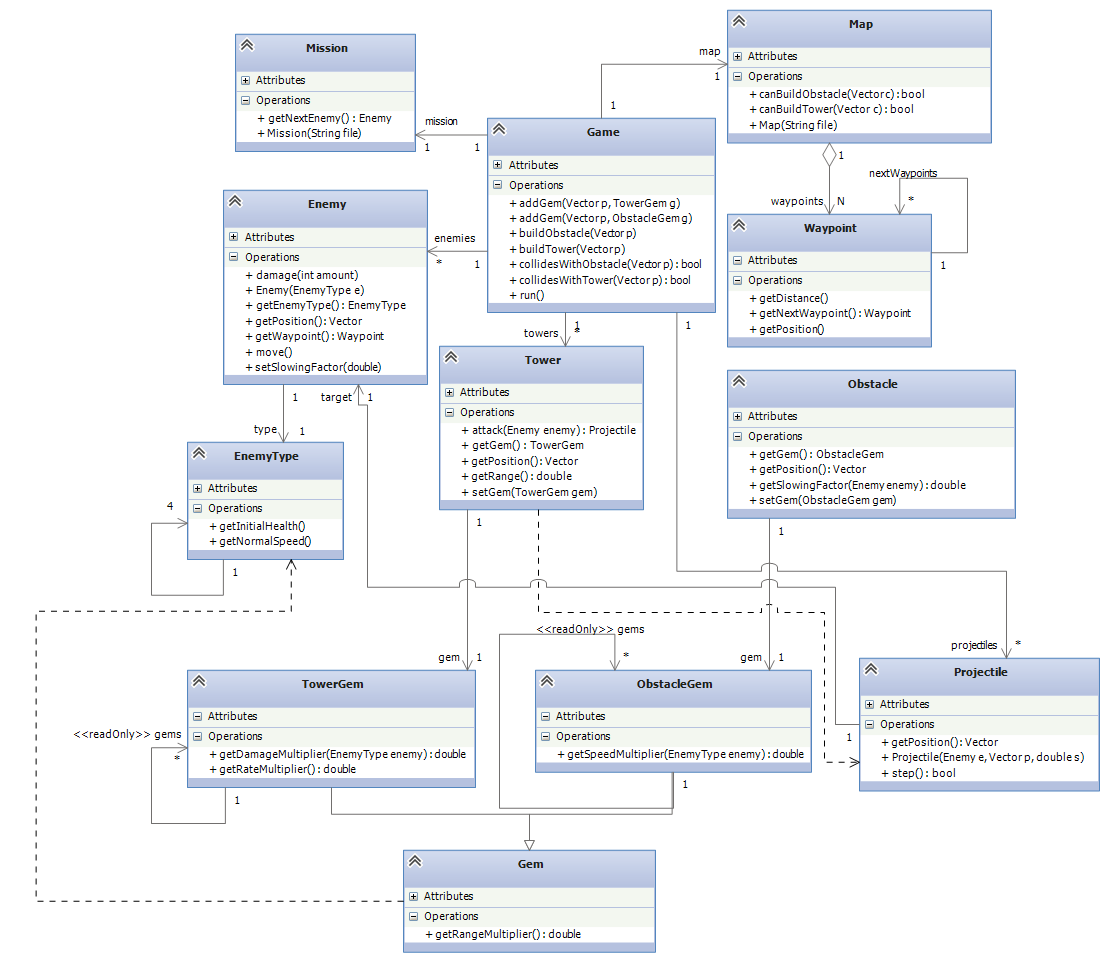
\includegraphics[width=177mm]{images/ch04/class.png}
\caption{Osztálydiagram}
\label{fig:class_diag}
\end{center}
\end{figure}


\section{Osztályok leírása}


\subsection{Enemy}
\begin{itemize}
\item Felelősség\\
Az ellenségek pozíciójának, sebességének és életerejének nyilvántartása.
\item Attribútumok
	\begin{itemize}
		\item \textbf{EnemyType} type: Az egység típusa.
		\item double health: Az ellenség fennmaradó életereje.
		\item \textbf{Vector} position: Pillanatnyi pozíció a pályán.
		\item \textbf{Waypoint} targetWaypoint: Az a \textbf{Waypoint}, ami felé az ellenség jelenleg tart.
		\item double slowingFactor: Az \textbf{EnemyType} sebességét ezzel kell beszorozni, hogy megkapjuk az ellenség tényleges jelenlegi sebességét.
	\end{itemize}
\item Metódusok
	\begin{itemize}
		\item Enemy(EnemyType et, Waypoint start): Létrehoz egy et typusú \textbf{Enemy}-t a start \textbf{Waypoint}-helyén.
		\item boolean move(): Az ellenséget a sebességének megfelelő mértékben mozgatja a célja irányába. Ha az ellenség életereje 0 vagy kisebb, akkor true-val tér visza, egyébként false-al.
		\item boolean damage(double amount): Csökkenti az ellenség életerejét amount-al, igazzal tér vissza ha az ellenség meghalt.
		\item \textbf{Vector} getPosition(): A position attribútum értékével tér vissza.
		\item \textbf{EnemyType} getEnemyType(): Visszaadja az ellenség típusát.
		\item double getDistance(): Visszaadja az ellenség céltól való távolságát a legrövidebb úton haladva.
		\item void setSlowingFactor(double sf): Beállítja a slowingFactor-t sf-re.
	\end{itemize}
\end{itemize}


\subsection{EnemyType}
\begin{itemize}
\item Felelősség\\
Leírja egy bizonyos típusú (fajú) ellenség alapvető tulajdonságait. Egy-egy példányára hivatkozik az összes ellenség, amelyeknek ezáltal meghatározza a viselkedését.
\item Attribútumok
	\begin{itemize}
		\item int cost: Az ilyen fajtájú ellenségek ára varázserőben.
		\item double initialHealth: Az ilyen fajtájú ellenségek kezdeti életereje.
		\item double normalSpeed: Az ilyen fajtájú ellenségek akadályoztatás nélküli haladási sebessége.
	\end{itemize}
\item Metódusok
	\begin{itemize}
		\item double getInitialHealth(): Visszaadja az initialHealth attribútum értékét.
		\item double getNormalSpeed(): Visszaadja a normalSpeed attribútum értékét.
	\end{itemize}
\end{itemize}




\subsection{Game}
\begin{itemize}
\item Felelősség\\
A többi osztály nyilván tartása és összekötése, a játékbeli események vezérlése. A felhasználói felülettől érkező parancsok végrehajtása, és a játék állapotának rendelkezésre bocsájtása a kijelzéshez.
\item Attribútumok
	\begin{itemize}
		\item List<\textbf{Projectile}> projectiles: Eltárolja a jelenleg játékban lévő lövedékeket.
		\item \textbf{Map} map: Referencia a kiválasztott pályára, amin a játék folyik.
		\item \textbf{Mission} mission: Referencia a kiválasztott misszióra, amely alapján zajlik a játék.
		\item List<\textbf{Tower}> towers: Eltárolja a játékos megépített tornyait.
		\item List<\textbf{Enemy}> enemies: Az összes jelenleg élő ellenség található meg benne.
		\item int magic: A játékos jelenlegi varázsereje.
	\end{itemize}
\item Metódusok
	\begin{itemize}
		\item void run(): Ez a metódus futtatja a főciklust, amelyben maga a játék működik.
		\item void buildTower(\textbf{Vector} position): Épít egy tornyot a paraméterül kapott helyen évő mezőre.
		\item void buildObstacle(\textbf{Vector} position): Épít egy akadályt a paraméterül kapott helyen lévő mezőre.
		\item void addGem(\textbf{Vector} position, \textbf{TowerGem} gem): A paraméterként kapott helyen lévő toronyra rárakja a paraméterként kapott varázskövet.
		\item void addGem(\textbf{Vector} position, \textbf{ObstacleGem} gem): A paraméterként kapott helyen lévő akadályra rárakja a paraméterként kapott varázskövet.
		\item boolean collidesWithTower(Vector p): megadja, hogy ha p helyre építenénk tornyot, az belelógna-e egy már megépített toronyba.
		\item boolean collidesWithObstacle(Vector p): megadja, hogy ha p helyre építenénk akadályt, az belelógna-e egy már megépített akadályba.
	\end{itemize}
\end{itemize}




\subsection{Gem}
\begin{itemize}
\item Felelősség\\
Egy általános varázskő tulajdonságainak tárolása.
\item Attribútumok
	\begin{itemize}
		\item int cost: A varázskő ára varázserőben.
		\item double rangeMultiplier: Megadja, hogy a varázskővel ellátott toronynak hányszorosára nő a hatótávolsága.
	\end{itemize}
\item Metódusok
	\begin{itemize}
		\item double getRangeMultiplier(): Visszaadja a varázskő hatótávolság szorzóját.
	\end{itemize}
\end{itemize}


\subsection{Map}
\begin{itemize}
\item Felelősség\\
Tartlamaz az összes \textbf{Waypoint} referenciát, felelős a kapott fájlból beolvasni a pályát, és felépíteni azt, valamint meg kell mondja, hogy van-e út a megadott \textbf{Vector}-nál.
\item Attribútumok
	\begin{itemize}
		\item List <\textbf{Waypoint}> waypoints: A pályán található \textbf{Waypoint}-ok listája.
	\end{itemize}
\item Metódusok
	\begin{itemize}
		\item Map(\textbf{String} file): Betölti a kapott elérési útvonalon a fájlt, és felépíti az alapján a pályát.
		\item bool canBuildObstacle(\textbf{Vector}): A \textbf{Waypoint}-ok alapján visszaadja, hogy lehet-e akadályt építeni a megadott helyen.
		\item bool canBuildTower(\textbf{Vector}): A \textbf{Waypoint}-ok alapján visszaadja, hogy lehet-e tornyot építeni a megadott helyen.
	\end{itemize}
\end{itemize}


\subsection{Mission}
\begin{itemize}
\item Felelősség\\
Felelőssége, felépíteni a listát, amely a beérkező ellenségeket és időzítésüket tartalmazza. Majd a megfelelő időközönként ki kell adja ezeket az egységeket a \textbf{Game} osztálynak.
\item Attribútumok
	\begin{itemize}
		\item \textbf{List}<\textbf{Spawn}> spawnList: A Spawn segédosztályban tárolt ellenség-idő-belépési pont, adatokat tárolja.
		\item double lastSpawn: Tárolja az előző spawn idejét.
	\end{itemize}
\item Metódusok
	\begin{itemize}
		\item Mission(\textbf{String} file): Betölti a kapott elérési útvonalon a fájlt, és felépíti az alapján a listát (spawnList).
		\item \textbf{Enemy} getNextEnemy(): A spawnList listaból a következő elemet megvizsgaálja, és ha spawnolni kell a következő ellenséget, akkor visszaadja azt.
	\end{itemize}
\end{itemize}


\subsection{Obstacle}
\begin{itemize}
\item Felelősség\\
Felelős, az ellenfelek lassításáért, úgy, hogy meg kell tudnia mondani a pozícióját, valamint, hogy az adott ellenséget mennyire lassítja.
\item Attribútumok
	\begin{itemize}
		\item \underline{int cost}: Az akadály ára varázserőben.
		\item \textbf{Gem} gem: Eltárol egy referenciát egy \textbf{Gem} típusú objektumra, ami meghatározza, hogy az adott épület milyen echant alatt áll.
		\item \textbf{Map}<\textbf{EnemyType}, double> slowingFactor: Megadja mekkora az adott típusú ellenfélre kifejtett hatása az akadálynak.
		\item \textbf{Vector} position: Az akadály koordinátáit tárolja.
	\end{itemize}
\item Metódusok
	\begin{itemize}
		\item int getCost(): Visszatér a cost attribútummal.
		\item double getSlowingFactor(\textbf{Enemy} enemy): Visszatér azzal az értékkel, amivel az adott ellenfelet lassítja.
		\item \textbf{Gem} getGem(): Visszaadja az épületen található varázskövet.
		\item void setGem(\textbf{Gem} gem): Beállítja az epületen lévő varázskövet. Ha már volt az épületen varázskő, akkor az előző megszűnik.
		\item \textbf{Vector} getPosition(): Visszaadja a position attribútumot.
	\end{itemize}
\end{itemize}


\subsection{ObstacleGem}
\begin{itemize}
\item Felelősség\\
Egy akadályra rakható varázskő tulajdonságainak tárolása.
\item Attribútumok
	\begin{itemize}
		\item HashMap<\textbf{EnemyType}, Double> speedMultiplier: Megadja, hogy a varázskővel elátott akadályon áthaladó adott típusú ellenség sebessége hányadára csökken.
	\end{itemize}
\item Metódusok
	\begin{itemize}
		\item double getSpeedMultiplier(\textbf{EnemyType} enemyType): Visszaadja varázskő sebesség szorzóját egy adott típusú ellenséghez.
	\end{itemize}
\end{itemize}


\subsection{Projectile}
\begin{itemize}
\item Felelősség\\
Követni a cél ellenséget, majd sebezni ha eléri.
\item Attribútumok
	\begin{itemize}
		\item double damage: A lövedék sebzése, ennyivel csökkenti a cél ellenség életerejét amikor eltalálja.
		\item \textbf{Vector} position: A lövedék pozíciója.
		\item double speed: A lövedék sebessége.
		\item \textbf{Enemy} enemy: A lövedék cél \textbf{Enemy}-je.
	\end{itemize}
\item Metódusok
	\begin{itemize}
		\item Projectile(\textbf{Enemy} enemy, \textbf{Vector} position, double speed): Konstruktor, átveszi a cél \textbf{Enemy}-t, a kezdő pozíciót és sebességet.
		\item boolean step():  speed-el mozgatja a lövedéket az ellenség irányába. Ha eltalálta az ellenséget vagy az ellenség már meghalt, akkor true-t ad vissza, különben false-t.
		\item \textbf{Vector} getPosition(): Visszaadja a lövedék pozícióját.
	\end{itemize}
\end{itemize}


\subsection{Tower}
\begin{itemize}
\item Felelősség\\
Felelős \textbf{Projectile}-ok létrehozásához, azok megfelelő felparaméterezésével. Továbbá felelős azért, hogy \textbf{Projectile}-okat csak a megadott időközönként lőjjön ki.
\item Attribútumok
	\begin{itemize}
		\item \underline{int cost}: A torony ára varázserőben.
		\item \textbf{Gem} gem: Eltárol egy referenciát egy \textbf{Gem} típusú objektumra, ami meghatározza, hogy az adott épület milyen echant alatt áll.
		\item \textbf{HashMap}<\textbf{EnemyType}, double> damage: Megadja mekkora az adott típusú ellenfélre kifejtett hatása a toronynak.
		\item \textbf{Vector} position: Visszatér az épület koordinátáival.
	\end{itemize}
\item Metódusok
	\begin{itemize}
		\item \textbf{Projectile} attack(List <\textbf{Enemy}>): Először megnézi, hogy lőhet-e, ha nem akkor NULL-t ad vissza. Ha igen akkor végignézi a kapott listában az ellenségeket, és amelyik a hatótávolságán belül van, és a legközelebb a célhoz, arra kilő egy \textbf{Projectile}-t, majd a visszatérési értékében visszaadja azt. A \textbf{Projectile}-t felparaméterezi az ellenséghez megfelelő sebzési adatokkal.
		\item int getCost(): Visszatér a cost attribútummal.
		\item \textbf{Gem} getGem(): Visszaadja az épületen található varázskövet.
		\item void setGem(\textbf{TowerGem} gem): Beállítja az epületen lévő varázskövet. Ha már volt az épületen varázskő, akkor az előző megszűnik.
		\item \textbf{Vector} getPosition(): Visszaadja a position attribútumot.
	\end{itemize}
\end{itemize}


\subsection{TowerGem}
\begin{itemize}
\item Felelősség\\
Egy toronyra rakható varázskő tulajdonságainak tárolása.
\item Attribútumok
	\begin{itemize}
		\item double rateMultiplier: Megadja, hogy a varázskővel ellátott toronynak hányszorosára nő a tüzelési sebessége.
		\item \textbf{HashMap}<\textbf{EnemyType}, \textbf{Double}> damageMultiplier: Megadja, hogy a varázskővel ellátott toronynak hányszorosára nő a sebzése egy adott típusú ellenséggel szemben.
	\end{itemize}
\item Metódusok
	\begin{itemize}
		\item double getRateMultiplier(): Visszaadja a varázskő tüzelési sebesség szorzójáz.
		\item double getDamageMultiplier(\textbf{EnemyType} enemyType): Visszaadja varázskő sebzés szorzóját egy adott típusú ellenséghez.
	\end{itemize}
\end{itemize}


\subsection{Waypoint}
\begin{itemize}
\item Felelősség\\
Útvonalat kijelölni az ellenségeknek, úgy, hogy megadja a pozícióját, amely felé az ellenségek mehetnek, valamint a következő  \textbf{Waypoint}-ot ami felé menniük kell, ha egyszer elérték ezt a  \textbf{Waypoint}-ot.
\item Attribútumok
	\begin{itemize}
		\item double distance: A  \textbf{Waypoint} távolságát a céltól tárolja.
		\item List <Waypoint, double> nextWaypoints: A következő  \textbf{Waypoint}-okat és a hozzájuk tartozó valószínűségeket tárolja el.
		\item \textbf{Vector} position: A  \textbf{Waypoint} helyét tárolja.
	\end{itemize}
\item Metódusok
	\begin{itemize}
		\item double getDistance(): Visszaadja a distance attribútumot.
		\item \textbf{Waypoint} getNextWaypoint(): Visszatér a nextWaypoints listából véletlenszerűen kiválasztott \textbf{Waypoint}-al
		\item\textbf{Vector} getPosition(): visszatér a position attribútummal.

	\end{itemize}
\end{itemize}



\section{Szekvencia diagramok}

\begin{figure}[H]
\begin{center}
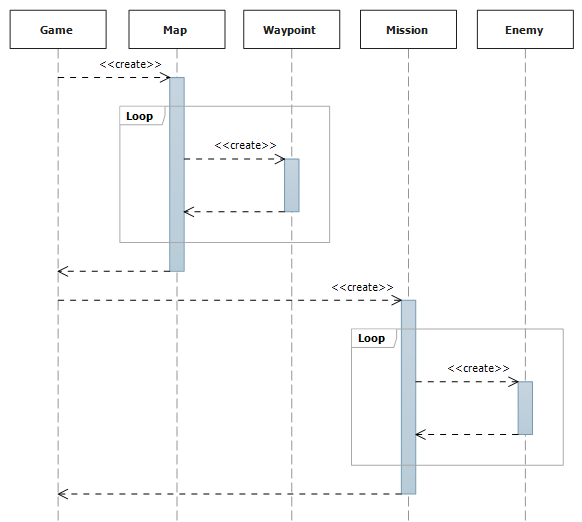
\includegraphics[width=15cm]{images/ch04/init.png}
\caption{Inicializálás. Betölti a mapet és a missiont.}
\label{fig:starting_game}
\end{center}
\end{figure}

\begin{figure}[H]
\begin{center}
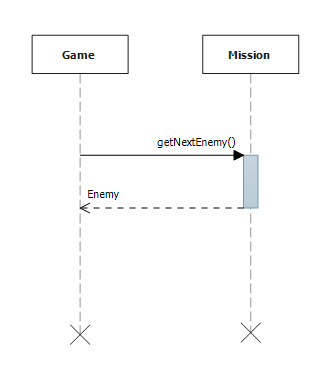
\includegraphics[width=8cm]{images/scheduling_enemies.png}
\caption{Ellenségek ütemezése.}
\label{fig:scheduling_enemies}
\end{center}
\end{figure}

\begin{figure}[H]
\begin{center}
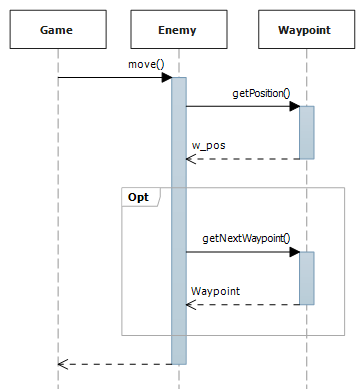
\includegraphics[width=10cm]{images/ch04/move_enemy.png}
\caption{Ellenség mozgatása. Ha elérte a waypointot lekéri a következőt.}
\label{fig:moving_enemy}
\end{center}
\end{figure}

\begin{figure}[H]
\begin{center}
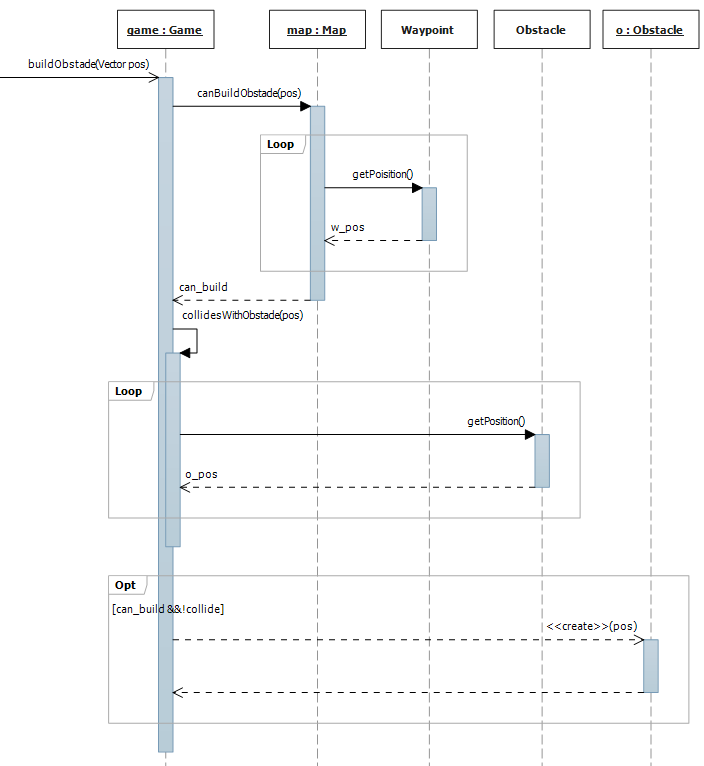
\includegraphics[width=480px]{images/ch04/build_obstacle.png}
\caption{Akadály építése. Megnézi, hogy szabad-e a helyre építeni, ha szabad épít.}
\label{fig:building_obstacle}
\end{center}
\end{figure}

\begin{figure}[H]
\begin{center}
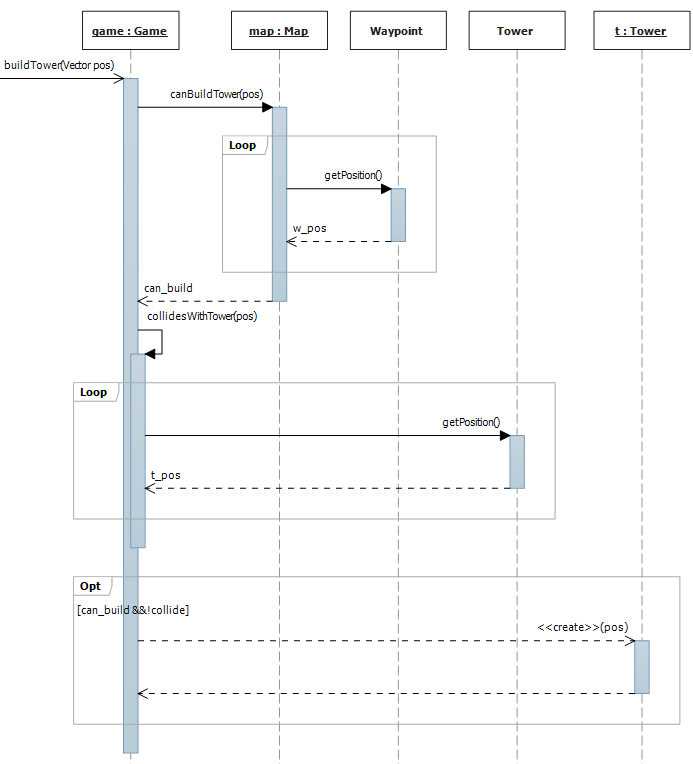
\includegraphics[width=480px]{images/ch04/build_tower.png}
\caption{Torony építése. Megnézi, hogy szabad-e a helyre építeni, ha szabad épít.}
\label{fig:building_tower}
\end{center}
\end{figure}

\begin{figure}[H]
\begin{center}
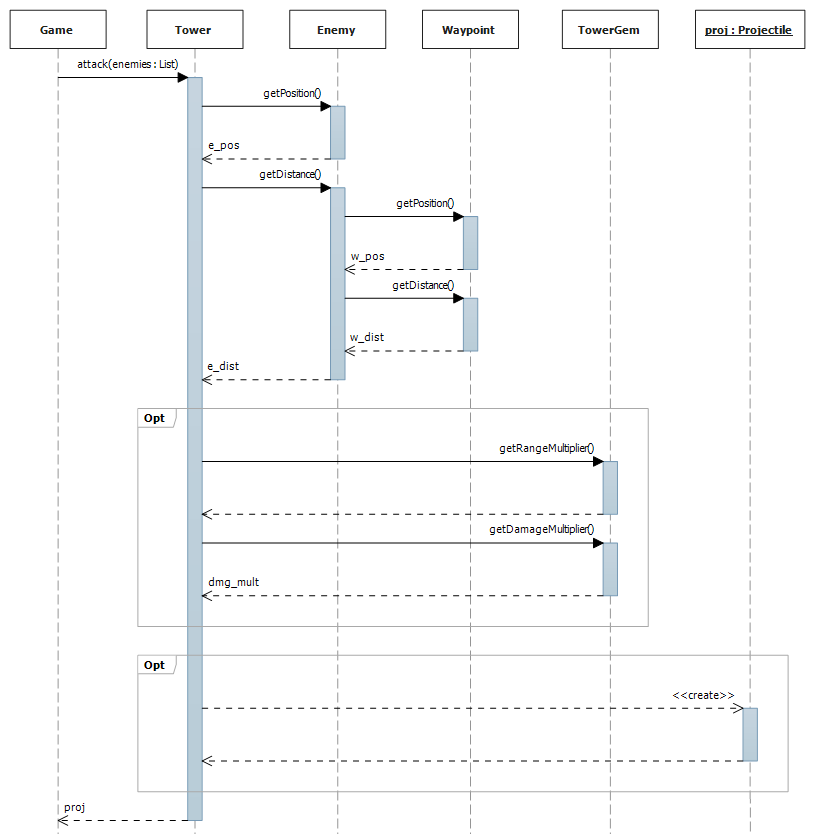
\includegraphics[width=17cm]{images/ch04/enemy_attack.png}
\caption{Ellenségek támadása. Minden ellenségre megnézi mennyire van távol a céltól és a legelsőre lő.}
\label{fig:tower_firing}
\end{center}
\end{figure}

\begin{figure}[H]
\begin{center}
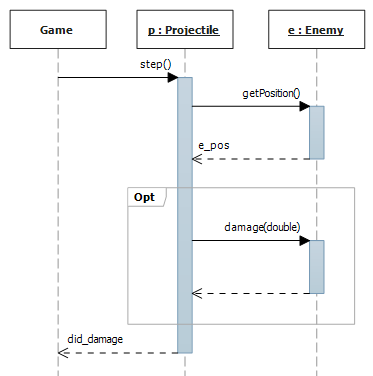
\includegraphics{images/ch04/projectile_step.png}
\caption{Lövedék léptetése.}
\label{fig:adding_gem}
\end{center}
\end{figure}

\begin{figure}[H]
\begin{center}
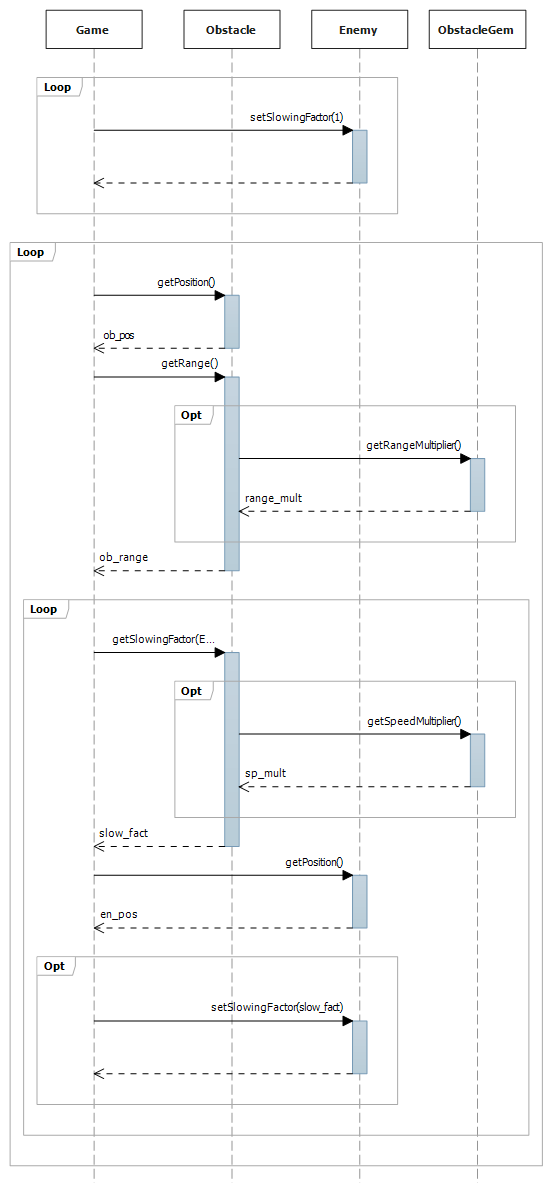
\includegraphics[width=14cm]{images/ch04/slow_enemy.png}
\caption{Minden akadály megnézi minden ellenségre, hogy a hatókörében van-e, ha igen lelassítja őket.}
\label{fig:adding_gem}
\end{center}
\end{figure}

\begin{figure}[H]
\begin{center}
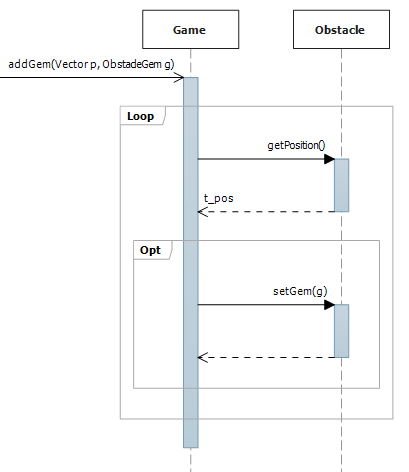
\includegraphics[width=92mm]{images/ch04/add_gem_obstacle.png}
\caption{Varázskő feltétele akadályra.}
\label{fig:adding_gem}

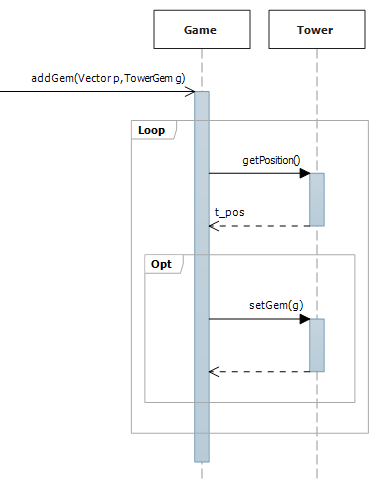
\includegraphics[width=92mm]{images/ch04/add_gem_tower.png}
\caption{Varázskő feltétele toronyra.}
\label{fig:adding_gem}
\end{center}
\end{figure}

\begin{figure}[H]
\begin{center}
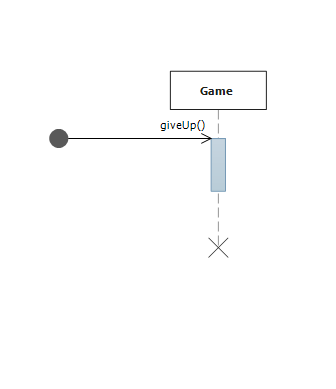
\includegraphics{images/giving_up.png}
\caption{Feladás.}
\label{fig:giving_up}
\end{center}
\end{figure}


\pagebreak
\section{State-chartok}

\begin{figure}[H]
\begin{center}
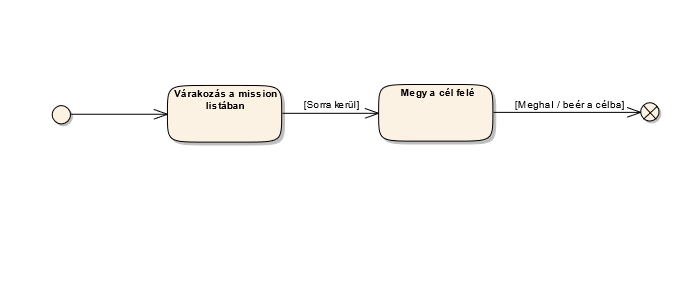
\includegraphics[width=15cm]{images/ch04/enemy_state.png}
\caption{Egy ellenség állapotdiagramja}
\label{fig:enemy_state}
\end{center}
\end{figure}

\begin{figure}[H]
\begin{center}
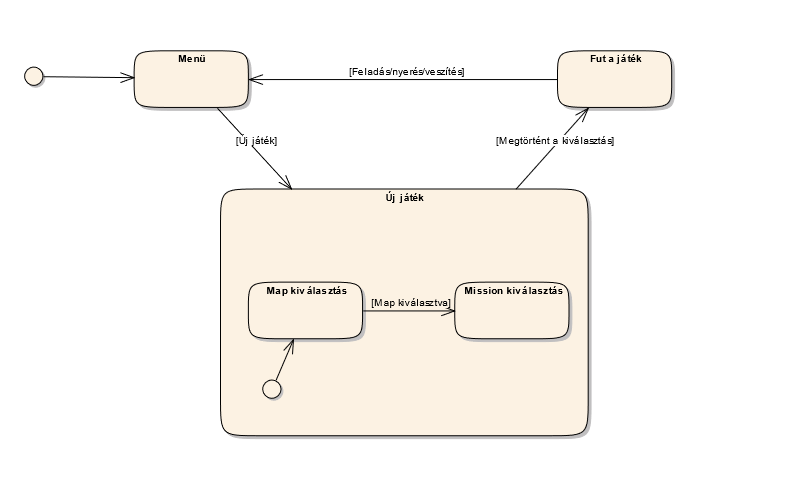
\includegraphics[width=15cm]{images/ch04/game_state.png}
\caption{A játék állapotdiagramja}
\label{fig:game_state}
\end{center}
\end{figure}

\begin{figure}[H]
\begin{center}
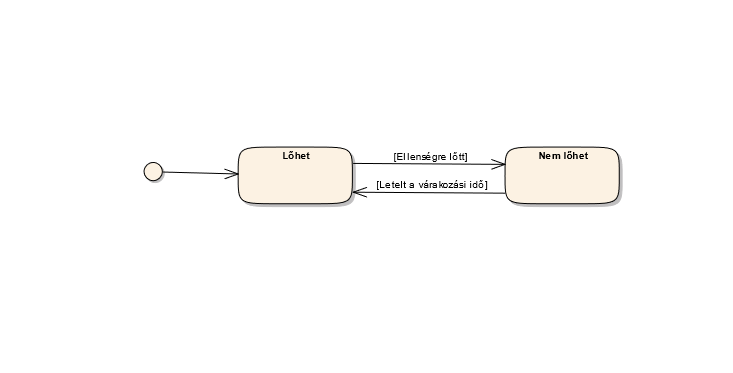
\includegraphics[width=15cm]{images/ch04/tower_state.png}
\caption{Egy torony állapotdiagramja}
\label{fig:tower_state}
\end{center}
\end{figure}


%\pagebreak
%% Szglab4
% ===========================================================================
%
\section{Napló}

\begin{naplo}


\bejegyzes
{2014.03.05.~8:00~} % Kezdet
{1,5 óra} % Időtartam
{\vadam\newline
\vantal\newline
\vbator\newline
\vtorok} % Résztvevők
{Kezdeti megbeszélés, hibák áttekintése.} % Leírás

\bejegyzes
{2014.03.09.~10:30~} % Kezdet
{4 óra} % Időtartam
{Tallér} % Résztvevők
{Szekvencia- és osztálydiagramok elkészítése.}

\bejegyzes
{2014.03.09.~17:00~}
{2 óra}
{\vadam}
{Map és Waypoint osztályok leírása, state chartok kijavítása.}

\bejegyzes
{...}
{...}
{...}
{...}


\end{naplo}


%%
%\setcounter{chapter}{4}
%% Szglab4
% ===========================================================================
%
\chapter{Szkeleton tervezése}

\thispagestyle{fancy}

\section{A szkeleton modell valóságos use-case-ei}
%\comment{A szkeletonnak, mint önálló programnak a működésével kapcsolatos use-case-ek.}

\subsection{Use-case diagram}

\begin{figure}[H]
\begin{center}
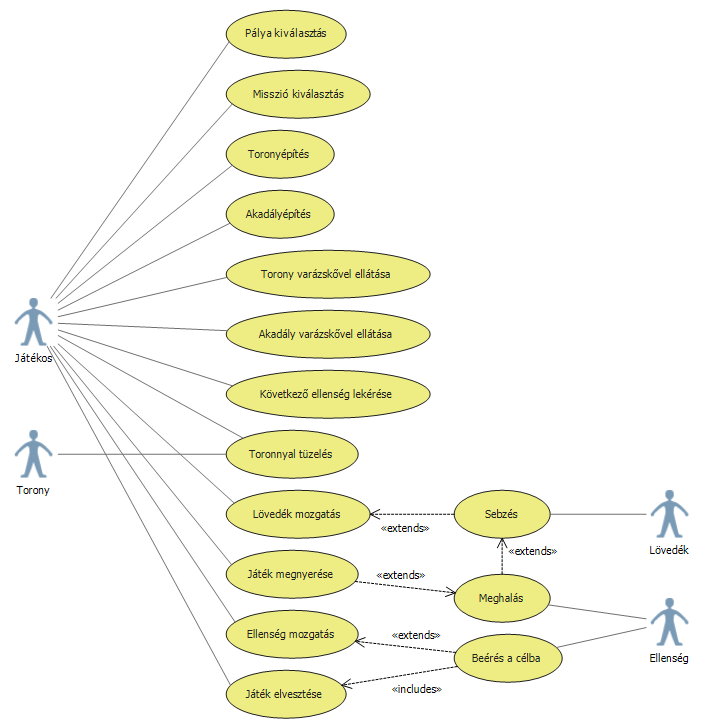
\includegraphics[width=17cm]{images/skeleton_use_case.png}
\caption{Use case diagram}
\label{fig:SzkeletonUseCase}
\end{center}
\end{figure}

\pagebreak

\subsection{Use-case leírások}
%\comment{Minden use-case-hez külön}

%Use-case neve  Rövid leírás  Aktorok  Forgatókönyv 

\usecase{Pálya kiválasztás}
{A felhasználó kiválaszt egy pályát.}
{Felhasználó}
{A program felkínál egy listát az elérhető pályák neveiről, amelyből a felhasználó kiválasztja azt, amelyiken játszani szeretne.}

\usecase{Misszió kiválasztás}
{A felhasználó kiválaszt egy missziót.}
{Felhasználó}
{A program felkínál egy listát az előzőleg kiválasztott pályán elérhető missziók neveiről, amelyből a felhasználó kiválasztja azt, amelyiken játszani szeretne.}

\usecase{Toronyépítés}
{A felhasználó felépít egy tornyot.}
{Felhasználó}
{A felhasználó megad egy pozíciót, ahova felépül egy torony.}

\usecase{Akadályépítés}
{A felhasználó felépít egy akadályt.}
{Felhasználó}
{A felhasználó megad egy pozíciót, ahova felépül egy akadály.}

\usecase{Torony varázskővel ellátása}
{A felhasználó ellát egy tornyot egy varászkővel.}
{Felhasználó}
{A felhasználó kiválaszt egy tornyot, majd egy varázskövet, amivel a toronyot erősíti.}

\usecase{Akadály varázskővel ellátása}
{A felhasználó ellát egy akadályt egy varázskővel.}
{Felhasználó}
{A felhasználó kiválaszt egy akadályt, majd egy varázskövet, amivel az akadályt erősíti.}

\usecase{Következő ellenség lekérése}
{A misszió következő ellensége elindul.}
{Felhasználó}
{A misszió soron következő ellensége létrejön, és elindul a pályán a célja felé.}

\usecase{Toronnyal tüzelés}
{Egy torony lő egyet.}
{Felhasználó, Torony}
{Egy kiválasztott torony kibocsát egy lövedéket egy megadott ellenség felé.}

\usecase{Ellenség mozgatás}
{Egy ellenség halad.}
{Ellenség}
{A kiválasztott ellenség megtesz egy lépést a célja felé vezető úton.}

\usecase{Beérés a célba}
{Egy ellenség elérte a célt.}
{Ellenség}
{Egy ellenség mozgása után elérte a célt, így a játéknak vége.}

\usecase{Játék elvesztése}
{A játék véget ér.}
{Játékos}
{A játék befejeződik, a játékos vesztett}

\usecase{Lövedék mozgatás}
{Egy lövedék halad.}
{Lövedék}
{A kiválasztott lövedék megtesz egy lépést a célpontja felé.}

\usecase{Sebzés}
{Egy lövedék célt ér.}
{Lövedék}
{Egy lövedék mozgása közben elérte a célpontját, azt megsebezte.}

\usecase{Meghalás}
{Egy ellenség életereje elfogy.}
{Ellenség}
{Ha egy lövedék célba érésekor az ellenségnek kevesebb életereje van, mint amennyit a lövedék sebez, az ellenség meghal, eltűnik.}

\usecase{Játék megnyerése}
{Az utolsó ellenség is meghal.}
{Játékos}
{Egy ellenség halálakor a játékos megnyeri a játékot, ha nincs több ellenség életben.}

\pagebreak
\setlength\parindent{15mm}
\section{A szkeleton kezelői felületének terve, dialógusok}
A szkeleton menüvezérelt módon fog működni. A felhasználónak meg kell adnia a kívánt parancsnak a kódját, majd a program lefuttatja azt. A program indítása után ki kell választani a pályát utána pedig a missziót. A menü felépítése itt látható: \\
\begingroup 
\fontsize{10pt}{10pt}\selectfont
\texttt{
1. Torony építés \\
\indent *1.1 Érvényes helyre akarunk építeni? I/N \\
\indent *1.2 Ütközik másik toronnyal? I/N \\
2. Akadály építés \\
\indent *2.1 Érvényes helyre akarunk építeni? I/N \\
\indent *2.2 Ütközik másik akadállyal? I/N \\
3. Következő ellenség lekérése \\
\indent *3.1 Van következő ellenség? I/N \\
4. Ellenség mozgatás \\
\indent *4.1 Elérte az ellenség a Waypointot? I/N \\
\indent *4.2 Hatósugarában van egy akadálynak? I/N \\
\indent \indent *4.2.1 Az akadályok van varázskő? I/N \\
5. Torony tüzelés \\
\indent *5.1 Van a torony hatósugarán belül ellenség? I/N \\
\indent \indent *5.1.1 Van a tornyon varázskő? I/N \\
6. Lövedék mozgatása \\
\indent *6.1 Elérte az ellenséget? I/N \\
7. Varázskő felrakása \\
\indent *7.1 Toronyra vagy akadályra? T/A \\
\indent *7.2 Érvényes helyet adtunk meg? I/N \\
8. Kilépés \\
\indent *8.1 Nyerés, vesztés, feladás vagy kilépés a programból? N/V/F/K \\
}
\endgroup \\
A *-gal jelölt menüpontokat nem lehet kiválasztani, ezt a program automatikusan megteszi, ha a felhasználó a parancs szülőjét meghívta. Ezek (1 kivétellel) igen/nem típusú kérdések. A kérdések végén láthatóak a lehetséges válaszok. A 8. pontnál  az N, V, F parancsok visszaléptetik a felhasználót a program elejére, tehát újra megkérdezi, hogy melyik pályát és missziót akarjuk kiválasztani.
\\
Az alábbi példa egy olyan interakciót mutat be, ahol a felhasználó építeni akar egy tornyot, ami érvényes helyen van, de ütközne egy másik toronnyal: \\
\begingroup
\fontsize{10pt}{10pt}\selectfont
\texttt{
? Adja meg a parancs kódját: 1 \\
- 1. Torony építése \\
>\indent ->[:Game].buildTower(pos): \\
>\indent \indent ->[:Map].canBuildTower(pos): \\
>\indent \indent \indent ->[:Waypoint].getPosition(): \\
?\indent \indent \indent 2.1. Érvényes a hely? I/N: I \\
<\indent \indent \indent <-[:Waypoint].getPosition() \\
<\indent \indent <-[:Map].canBuildTower(): \\
>\indent \indent ->[:Game].collidesWithTower(pos): \\
>\indent \indent \indent ->[:Tower].getPosition(): \\
?\indent \indent \indent 2.2. Ütközik másik toronnyal? I/N: I \\
<\indent \indent \indent <-[:Tower].getPosition() \\
>\indent \indent <-[:Game].collidesWithTower(pos) \\
>\indent <-[:Game].buildTower() \\
? Adja meg a parancs kódját:
} \\
\endgroup
\pagebreak
Minden sor elején van 1 karakter, ami a sor típusát jelöli.
\begin{itemize}
\item '?': kérdés, felhasználói interakcióra vár
\item '-': megjegyzés
\item '>': metódusba lépés
\item '<': metódusból visszatérés
\end{itemize}
A metódusba lépéskor és visszatérésnél, egy nyíl jelöli, hogy hívásról vagy visszatérésról van-e szó majd szögletes zárójelek között található az objektum típusa, ezután pedig a metódus neve. Például: ->[:Osztály].metódus():

\section{Szekvencia diagramok a belső működésre}
Az előző fejezetben lévő szekvencia diagramok továbbra is érvényesek. \\
\begin{figure}[H]
\begin{center}
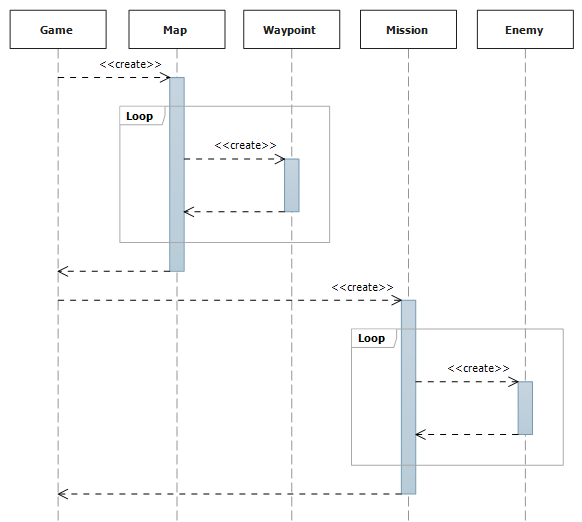
\includegraphics[width=15cm]{images/ch04/init.png}
\caption{Inicializálás. Betölti a mapet és a missiont.}
\label{fig:starting_game}
\end{center}
\end{figure}

\begin{figure}[H]
\begin{center}
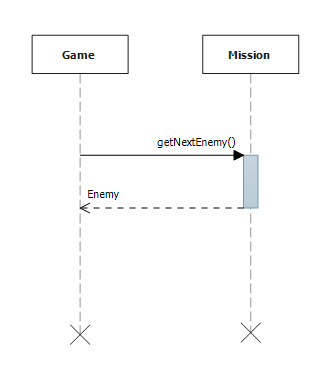
\includegraphics[width=8cm]{images/scheduling_enemies.png}
\caption{Ellenségek ütemezése.}
\label{fig:scheduling_enemies}
\end{center}
\end{figure}

\begin{figure}[H]
\begin{center}
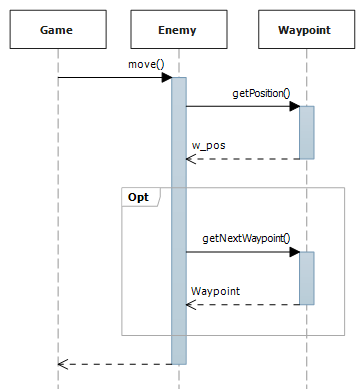
\includegraphics[width=10cm]{images/ch04/move_enemy.png}
\caption{Ellenség mozgatása. Ha elérte a waypointot lekéri a következőt.}
\label{fig:moving_enemy}
\end{center}
\end{figure}

\begin{figure}[H]
\begin{center}
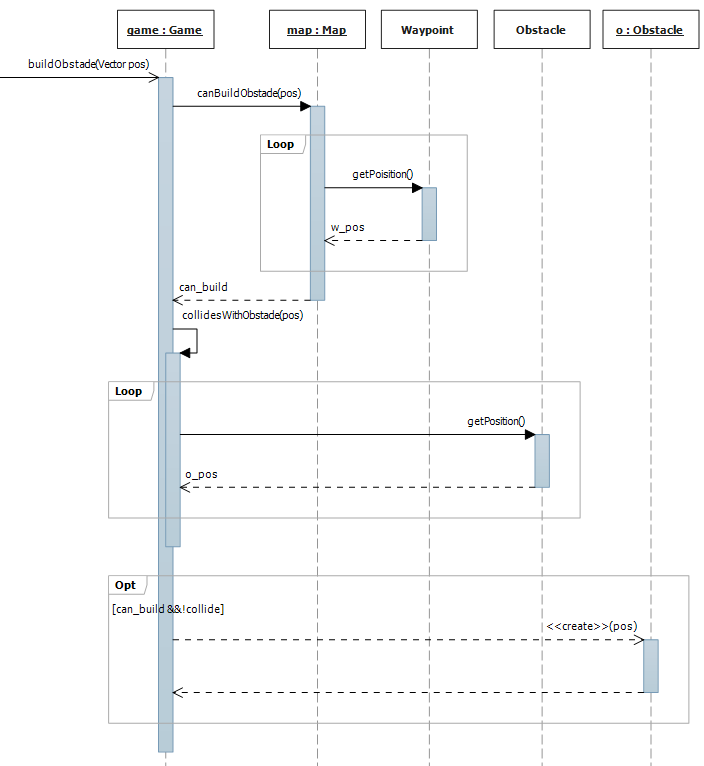
\includegraphics[width=480px]{images/ch04/build_obstacle.png}
\caption{Akadály építése. Megnézi, hogy szabad-e a helyre építeni, ha szabad épít.}
\label{fig:building_obstacle}
\end{center}
\end{figure}

\begin{figure}[H]
\begin{center}
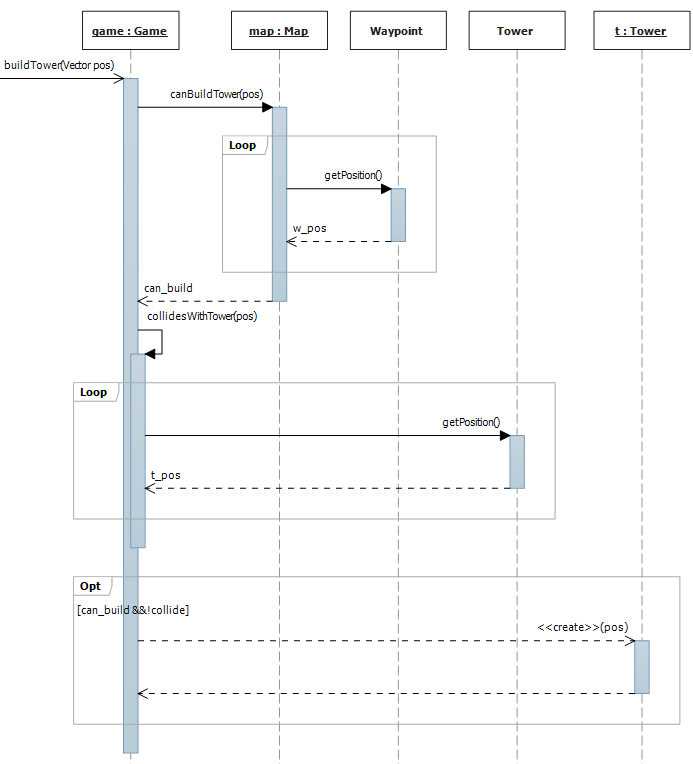
\includegraphics[width=480px]{images/ch04/build_tower.png}
\caption{Torony építése. Megnézi, hogy szabad-e a helyre építeni, ha szabad épít.}
\label{fig:building_tower}
\end{center}
\end{figure}

\begin{figure}[H]
\begin{center}
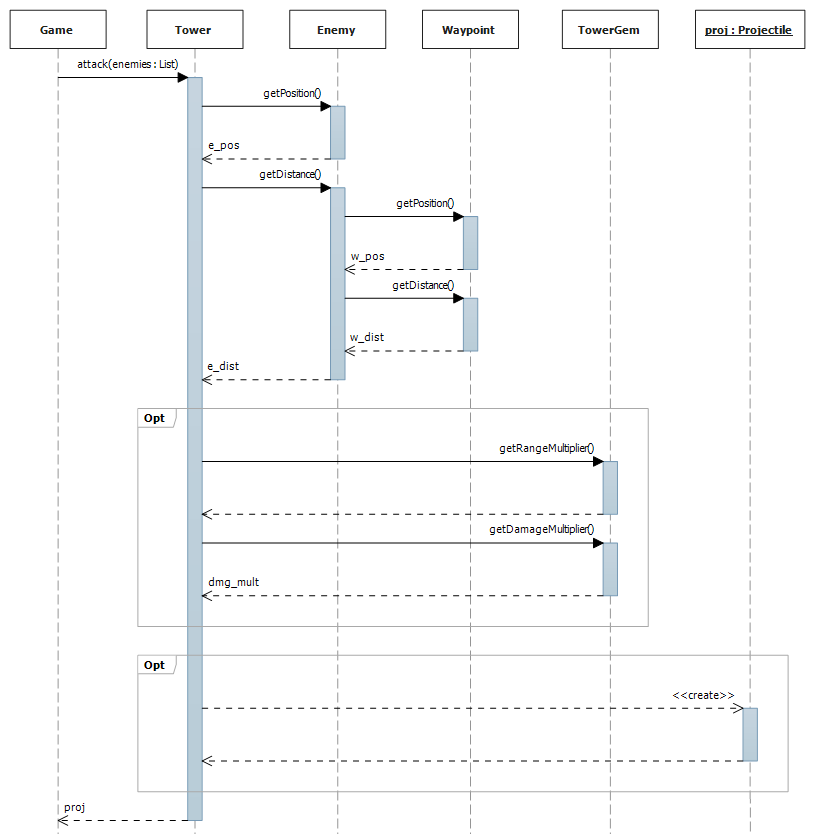
\includegraphics[width=17cm]{images/ch04/enemy_attack.png}
\caption{Ellenségek támadása. Minden ellenségre megnézi mennyire van távol a céltól és a legelsőre lő.}
\label{fig:tower_firing}
\end{center}
\end{figure}

\begin{figure}[H]
\begin{center}
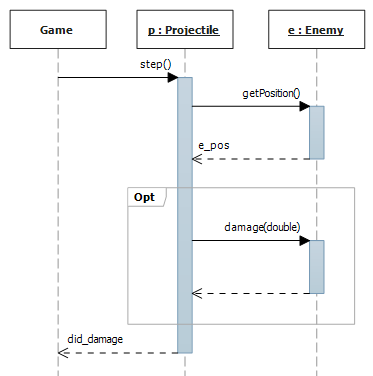
\includegraphics{images/ch04/projectile_step.png}
\caption{Lövedék léptetése.}
\label{fig:adding_gem}
\end{center}
\end{figure}

\begin{figure}[H]
\begin{center}
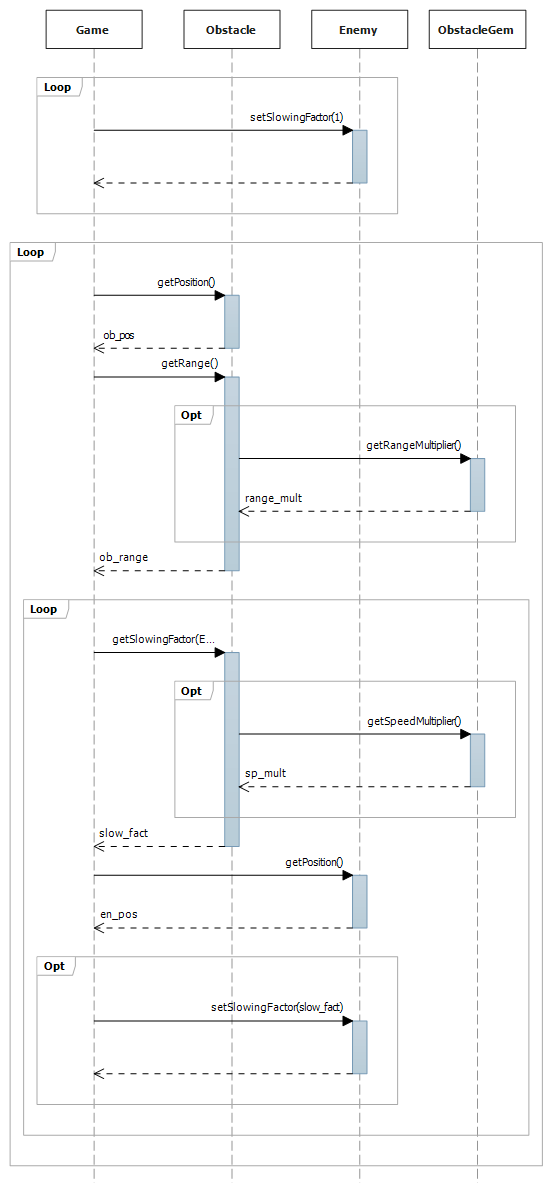
\includegraphics[width=14cm]{images/ch04/slow_enemy.png}
\caption{Minden akadály megnézi minden ellenségre, hogy a hatókörében van-e, ha igen lelassítja őket.}
\label{fig:adding_gem}
\end{center}
\end{figure}

\begin{figure}[H]
\begin{center}
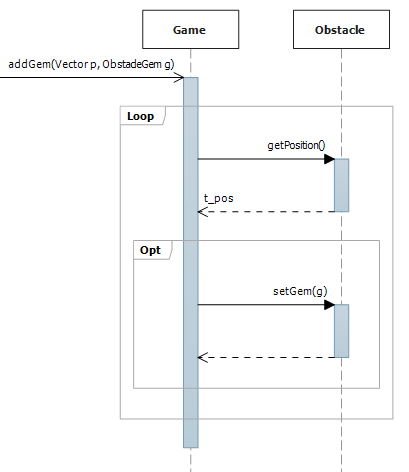
\includegraphics[width=92mm]{images/ch04/add_gem_obstacle.png}
\caption{Varázskő feltétele akadályra.}
\label{fig:adding_gem}

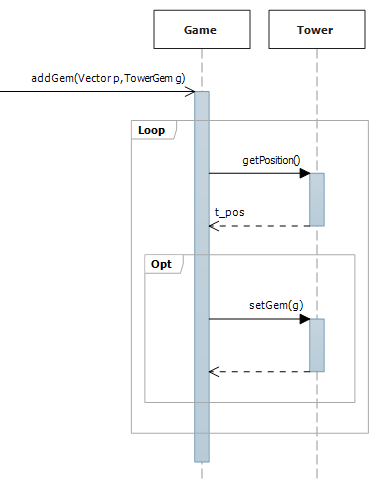
\includegraphics[width=92mm]{images/ch04/add_gem_tower.png}
\caption{Varázskő feltétele toronyra.}
\label{fig:adding_gem}
\end{center}
\end{figure}

\begin{figure}[H]
\begin{center}
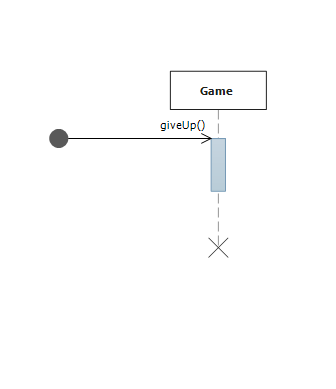
\includegraphics{images/giving_up.png}
\caption{Feladás.}
\label{fig:giving_up}
\end{center}
\end{figure}


\pagebreak

\section{Kommunikációs diagramok}
%\comment{A szkeletonban, az egyes szkeleton-use-case-ek futása során létrehozott objektumok és kapcsolataik bemutatására szolgáló %diagramok. Ezek alapján valósítják meg a szkeleton fejlesztői az inicializáló kódrészleteket.}

\begin{figure}[H]
\begin{center}
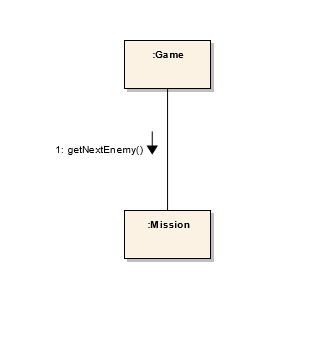
\includegraphics{images/ch05/nextEnemyKomm.png}
\caption{Ellenségek ütemezése.}
\label{fig:nextEnemyKomm}
\end{center}
\end{figure}

\begin{figure}[H]
\begin{center}
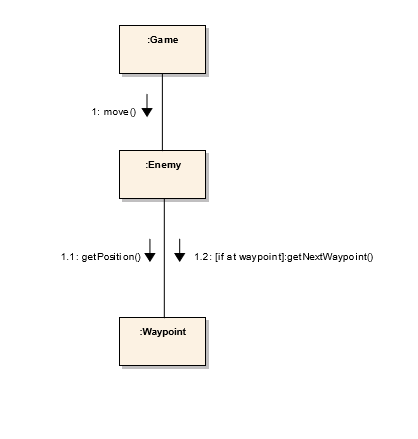
\includegraphics{images/ch05/moveKomm.png}
\caption{Ellenség mozgatása.}
\label{fig:moveKomm}
\end{center}
\end{figure}

\begin{figure}[H]
\begin{center}
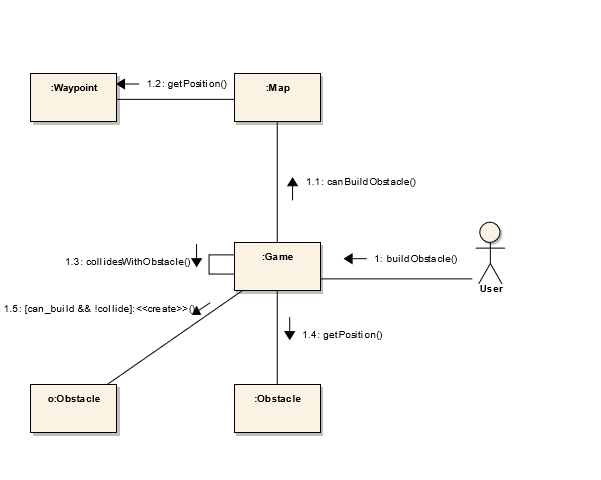
\includegraphics{images/ch05/buildObKomm.png}
\caption{Akadály építése.}
\label{fig:buildObKomm}
\end{center}
\end{figure}

\begin{figure}[H]
\begin{center}
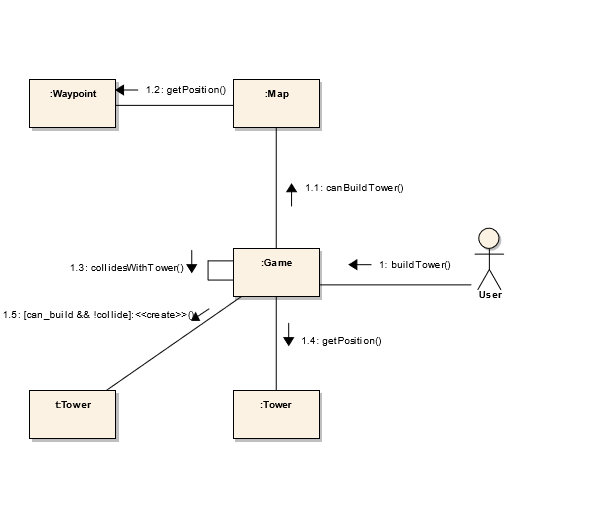
\includegraphics{images/ch05/buildTowerKomm.png}
\caption{Torony építése.}
\label{fig:buildTowerKomm}
\end{center}
\end{figure}

\begin{figure}[H]
\begin{center}
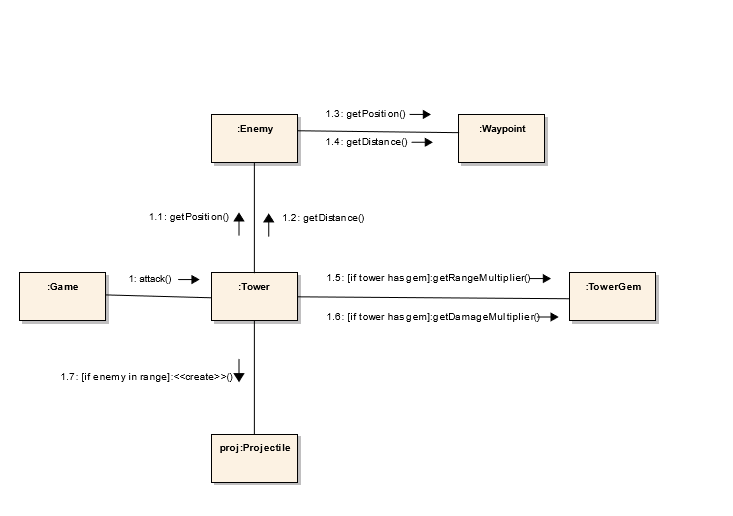
\includegraphics{images/ch05/attackKomm.png}
\caption{Torony tüzelése egy ellenségre.}
\label{fig:attackKomm}
\end{center}
\end{figure}

\begin{figure}[H]
\begin{center}
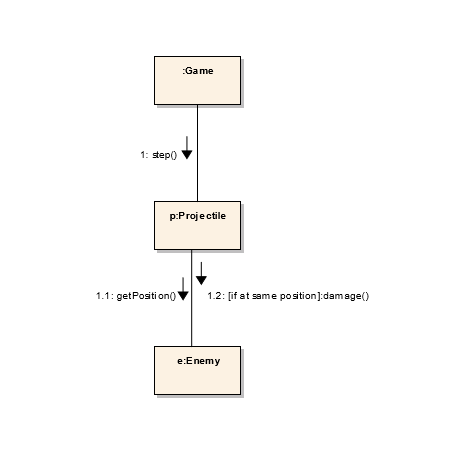
\includegraphics{images/ch05/projectileMoveKomm.png}
\caption{Lövedék mozgatása.}
\label{fig:projectileMoveKomm}
\end{center}
\end{figure}

\begin{figure}[H]
\begin{center}
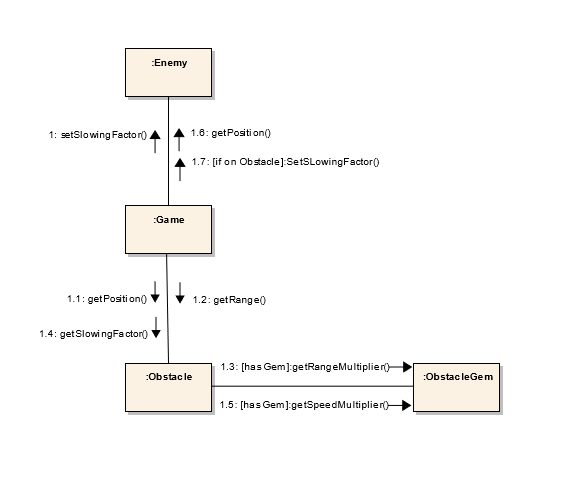
\includegraphics{images/ch05/slowKomm.png}
\caption{Akadályon áthaladó ellenség lassítása.}
\label{fig:slowKomm}
\end{center}
\end{figure}

\begin{figure}[H]
\begin{center}
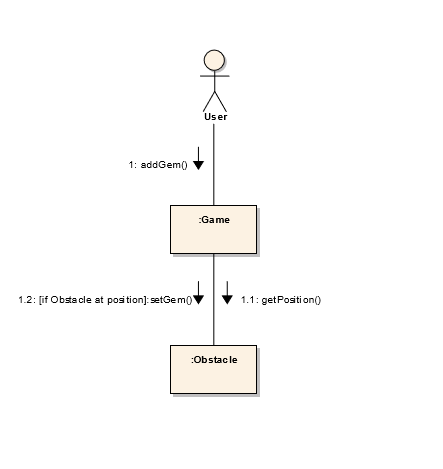
\includegraphics{images/ch05/addGemToObKomm.png}
\caption{Varázskő feltétele akadályra.}
\label{fig:addGemToObKomm}
\end{center}
\end{figure}


\begin{figure}[H]
\begin{center}
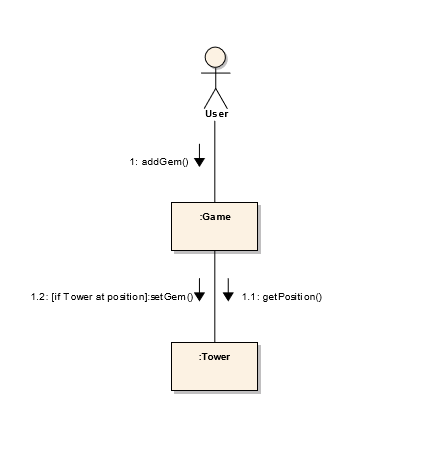
\includegraphics{images/ch05/addGemToTowerKomm.png}
\caption{Varázskő feltétele toronyra.}
\label{fig:addGemToTowerKomm}
\end{center}
\end{figure}

%% Szglab4
% ===========================================================================
%
\section{Napló}

\begin{naplo}

\bejegyzes
{2014.03.16.~19:00~}
{1 óra}
{\vadam\newline
\vantal\newline
\vbator\newline
\vtorok}
{Értekezlet. Döntés: Nusser elkészíti a kommunikációs diagramokat. Szabó elkészíti a use case diagramot. Török elkészíti a use case-ek szöveges leírását.}

\bejegyzes
{2014.03.16.~20:00~}
{2 óra}
{\vtorok}
{Tevékenység: \vtorok leírja a szkeleton use case-eit.}

%\bejegyzes
%{...}
%{...}
%{...}
%{...}


\end{naplo}


%%
%\setcounter{chapter}{5}
%% Szglab4
% ===========================================================================
%
\chapter{Szkeleton beadás}

\thispagestyle{fancy}

\section{Fordítási és futtatási útmutató}

\subsection{Fájllista}

\begin{fajllista}

\fajl
{Enemy.java} % Kezdet
{1 967 byte} % Idptartam
{2014.03.20~10:51~}
{Enemy osztály.} % Leírás

\fajl
{EnemyType.java} % Kezdet
{530 byte} % Idptartam
{2014.03.21~22:53~}
{EnemyType osztály.} % Leírás

\fajl
{Game.java} % Kezdet
{9 606 byte} % Idptartam
{2014.03.20~9:25~}
{Game osztály. Innen indul a program.} % Leírás

\fajl
{Gem.java} % Kezdet
{403 byte} % Idptartam
{2014.03.21~22:53~}
{Gem osztály.} % Leírás

\fajl
{Map.java} % Kezdet
{926 byte} % Idptartam
{2014.03.20~10:51~}
{Map osztály.} % Leírás

\fajl
{Mission.java} % Kezdet
{771 byte} % Idptartam
{2014.03.20~10:51~}
{Mission osztály.} % Leírás

\fajl
{Obstacle.java} % Kezdet
{1 693 byte} % Idptartam
{2014.03.21~22:53~}
{Obstacle osztály.} % Leírás

\fajl
{ObstacleGem.java} % Kezdet
{599 byte} % Idptartam
{2014.03.20~10:32~}
{ObstacleGem osztály.} % Leírás

\fajl
{Projectile.java} % Kezdet
{1 165 byte} % Idptartam
{2014.03.20~10:51~}
{Projectile osztály.} % Leírás

\fajl
{Tower.java} % Kezdet
{2 085 byte} % Idptartam
{2014.03.20~10:51~}
{Tower osztály.} % Leírás

\fajl
{TowerGem.java} % Kezdet
{575 byte} % Idptartam
{2014.03.20~10:32~}
{TowerGem osztály.} % Leírás

\fajl
{Vector.java} % Kezdet
{50 byte} % Idptartam
{2014.03.20~10:31~}
{Vector segédosztály.} % Leírás

\fajl
{Waypoint.java} % Kezdet
{853 byte} % Idptartam
{2014.03.21~22:53~}
{Waypoint osztály.} % Leírás

\end{fajllista}

\subsection{Fordítás}

\lstset{escapeinside=`', xleftmargin=10pt, frame=single, basicstyle=\ttfamily\footnotesize, language=sh}
\begin{lstlisting}
javac -d bin src/szoftlab4/*.java
\end{lstlisting}

\subsection{Futtatás}

\lstset{escapeinside=`', xleftmargin=10pt, frame=single, basicstyle=\ttfamily\footnotesize, language=sh}
\begin{lstlisting}
cd bin
java szoftlab4.Game
\end{lstlisting}

\section{Értékelés}

\begin{ertekeles}
\tag{Nusser} % Tag neve
{24}        % Munka szazalekban
\tag{Szabó}
{27}
\tag{Tallér}
{34}
\tag{Török}
{16}
\end{ertekeles}

\section{Módosítások}
\subsection{Menü}
A 7. Varázskő felrakása menüpontba raktunk egy *7.2 Érvényes helyet adtunk meg? kérdést. \\
Egy új menüpontot raktunk a programba \\
8. Ellenségek lassítása \\
*8.1 Van varázskő az akadályon (I/N)? \\
*8.2 Van ellenség az akadály hatókörében (I/N)? \\
Ezzel együtt a 8. Kilépés menüpont, 9. Kilépésre változott. \\

\subsection{Game osztály}
A Game.run metódus visszatérési értékét boolean-ra változtattuk. Igazzal tér vissza ha a játékos nyert/vesztett/feladata, hamissal tér vissza ha kilép a játékból.

\subsection{Obstacle}
Az Obstacle-ből kimaradt a getRange() metódus, ami az osztálydiagramban és az osztály leírásánál nem szerepel, de a szekvencia diagramokban igen. A metódus visszaadja az akadály hatótávolságát.

%% Szglab4
% ===========================================================================
%
\section{Napló}

\begin{naplo}

\bejegyzes
{2014.03.20.~9:00~} % Kezdet
{2 óra} % Időtartam
{Tallér} % Résztvevők
{Szekvencia kiíró metódusok megírása. Game osztály kódolása.}

\bejegyzes
{2014.03.21.~22:00~} % Kezdet
{1 óra} % Időtartam
{Tallér} % Résztvevők
{Game osztály befejezése. Menü befejezése.}

\bejegyzes
{2014.03.22.~17:00~} % Kezdet
{1 óra} % Időtartam
{Török} % Résztvevők
{A Tower, Obstacle, Gem és ObstacleGem osztályok metódusainak létrehozása, dokumentálása.}

\bejegyzes
{2010.03.23.~23:00~}
{5 óra}
{Németh}
{Tevékenység: Németh implementálja a tesztelő programokat.}


\end{naplo}


%%
%\setcounter{chapter}{6}
%% Szglab4
% ===========================================================================
%
\chapter{Prototípus koncepciója}

\thispagestyle{fancy}
\setcounter{section}{0}
\section{Változások a specifikációban}

\subsection{Köd}
\textbf{A tornyokra időnként köd ereszkedik, aminek következtében a látás erősen lecsökken. Ez hatással van a lövésre.}\\
Egy új Fog osztályt vezetünk be. Ennek van egy darab statikus getRangeMultiplier() metódusa, ami visszaadja mennyivel csökkenjen a látótáv, valamint van egy setFog(bool), amivel be lehet állítani, hogy van-e köd vagy nincs. Ha nincs köd beállítva getRangeMultiplier() 1-et ad vissza.

\subsection{Elágazások}
\textbf{A játékosok által járható útvonalon lehetnek elágazások és becsatlakozások. Az elágazásokon az egyes játékosok véletlenszerűen mennek a különböző irányokba.}\\
Mi a feladatot alapból így specifikáltuk, ezért változásra nincs szükség.
\subsection{Új lövedék}
\textbf{A tornyokban elvétve lehetnek olyan lövedékek, amelyek az eltalált játékost kettőbe vágják. A két játékos egymástól függetlenül él tovább, csökkentett életerővel.}\\
Ehhez létrehoztunk egy új SplitterProjectile osztályt, ami a Projectile osztályból származik le. Valamint hozzáadtunk az Enemy osztályhoz egy split() metódust. A Game osztályhoz pedig egy addEnemy(Enemy) metódust adtunk, amit a SplitterProjectile hív meg egy callback-el, amikor kettévágta az ellenséget.

\subsection{Módosult osztálydiagram}
\begin{figure}[H]
\begin{center}
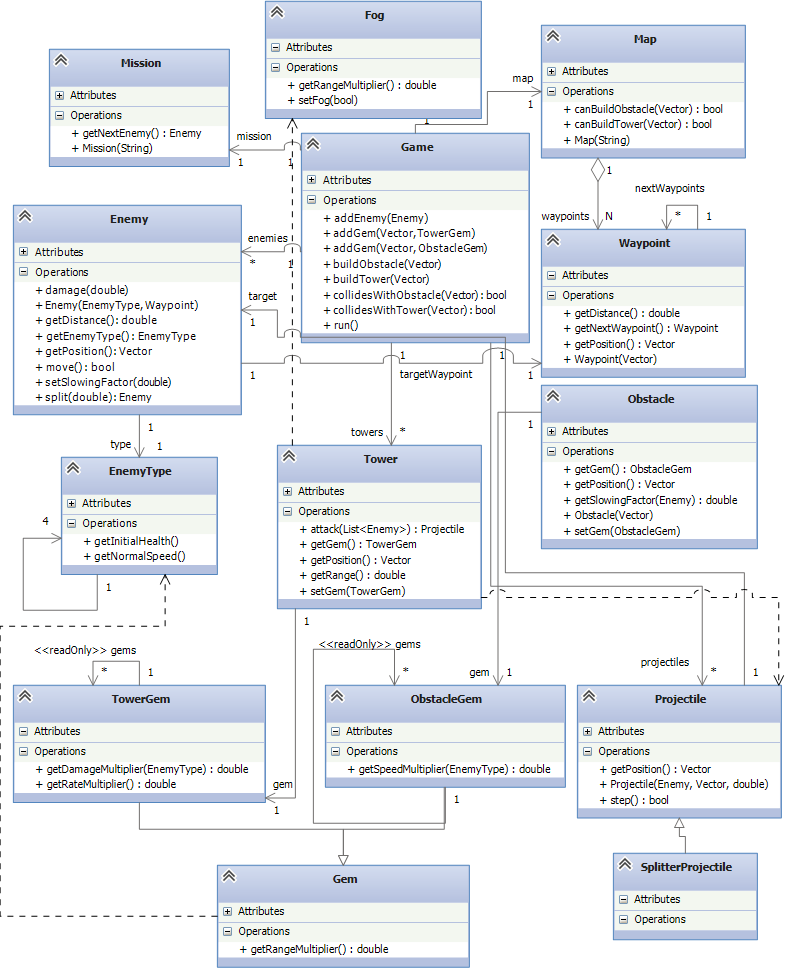
\includegraphics[width=17cm]{images/ch07/class_new.png}
\caption{Osztály diagram}
\label{fig:classDiagNew}
\end{center}
\end{figure}

\subsection{Módosult szekvencia diagramok}
\begin{figure}[H]
\begin{center}
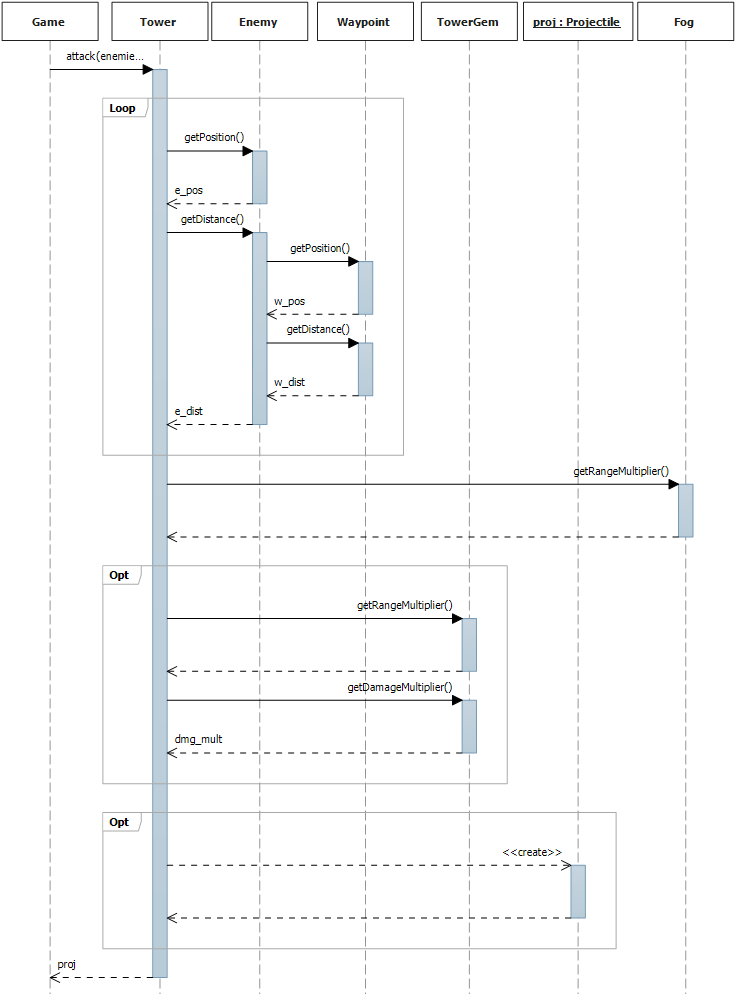
\includegraphics[width=17cm]{images/ch07/attack_enemy.png}
\caption{Ellenség támadása}
\label{fig:enemyAttackNew}
\end{center}
\end{figure}

\begin{figure}[H]
\begin{center}
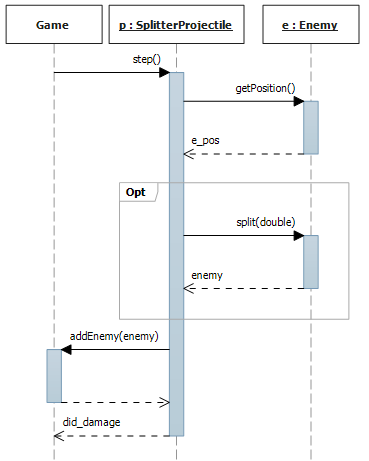
\includegraphics[width=10cm]{images/ch07/splitterprojectile_step.png}
\caption{Újfajta lövedék mozgatása}
\label{fig:splitProjMove}
\end{center}
\end{figure}


\section{Prototípus interface-definíciója}
%\comment{Definiálni kell a teszteket leíró nyelvet. Külön figyelmet kell fordítani arra, hogy ha a rendszer véletlen elemeket is tartalmaz, akkor a véletlenszerűség ki-bekapcsolható legyen, és a program determinisztikusan is tesztelhető legyen.}

\subsection{Az interfész általános leírása}
%\comment{A protó (karakteres) input és output felületeit úgy kell kialakítani, hogy az input fájlból is vehető legyen illetőleg az output fájlba menthető legyen, vagyis kommunikációra csak a szabványos be- és kimenet használható.}

Az interfész csak a szabványos bemenetről fogad parancsokat, és a szabványos kimenetre írja ki az esetleges kimenetet. Ezáltal terminálból is használható, valamint az elkészítendő tesztelő segédprogram segítségével átirányítható a ki- és bemenet fájlokra, így van mód automatikus tesztelésre, előre elkészített teszteseteket felhasználva. A tesztesetek a prototípusnak adandó parancsok sorozatából, valamint az adott sorozatra adandó helyes kimenet található. A tesztek sikeresek, ha a valós, és a leírt elvárt kimenet megegyezik.

\subsection{Bemeneti nyelv}
%\comment{Definiálni kell a teszteket leíró nyelvet. Külön figyelmet kell fordítani arra, hogy ha a rendszer véletlen elemeket is tartalmaz, akkor a véletlenszerűség ki-bekapcsolható legyen, és a program determinisztikusan is futtatható legyen. A szálkezelést is tesztelhető, irányítható módon kell megoldani.}

A prototípus által elfogadott parancsok a következők:

\begin{itemize}

\item loadMap
	\begin{itemize}
	\item Leírás: Egy pálya betöltése
	\item Opciók: A betöltendő pálya neve
	\end{itemize}

\item loadMission
	\begin{itemize}
	\item Leírás: Egy misszió betöltése
	\item Opciók: A betöltendő misszió neve
	\end{itemize}

\item setFog
	\begin{itemize}
	\item Leírás: A köd beállítása
	\item Opciók: A köd kívánt állapota: 0 - nincs köd, 1 - van köd
	\end{itemize}

\item setCritical
	\begin{itemize}
	\item Leírás: A kettévágó lövedék beállítása
	\item Opciók: A kívánt hatás: 0 - nem kettévágó lövedék, 1 - kettévágó lövedék
	\end{itemize}

\item setWaypoint
	\begin{itemize}
	\item Leírás: A csomópontokból való továbbhaladás irányának beállítása
	\item Opciók: A következő csomópont azonosítója
	\end{itemize}

\item step
	\begin{itemize}
	\item Leírás: A játéklogika léptetése
	\item Opciók: A léptetni kívánt időegységek száma
	\end{itemize}

\item buildTower
	\begin{itemize}
	\item Leírás: Toronyépítés
	\item Opciók: Az építendő torony koordinátái
	\end{itemize}

\item buildObstacle
	\begin{itemize}
	\item Leírás: Akadály építése
	\item Opciók: Az építendő akadály koordinátái
	\end{itemize}

\item enchant
	\begin{itemize}
	\item Leírás: Torony vagy akadály felszerelése drágakővel
	\item Opciók: A drágakő típusa, illetve a felszerelendő épület koordinátái
	\end{itemize}

\item listEnemies
	\begin{itemize}
	\item Leírás: A pályán lévő ellenségek kilistázása
	\item Opciók: -
	\end{itemize}

\item listTowers
	\begin{itemize}
	\item Leírás: A tornyok kilistázása
	\item Opciók: -
	\end{itemize}

\item listObstacles
	\begin{itemize}
	\item Leírás: Az akadályok kilistázása
	\item Opciók: -
	\end{itemize}

\item listProjectiles
	\begin{itemize}
	\item Leírás: A lövedékek kilistázása
	\item Opciók: -
	\end{itemize}


\end{itemize}

%\comment{Ha szükséges, meg kell adni a konfigurációs (pl. pályaképet megadó) fájlok nyelvtanát is.}

A pályákat és missziókat leíró fájlok XML formátumban lesznek, a következő DTD-k szerint:\newline
\newline
<!DOCTYPE map\newline
[\newline
<!ELEMENT map (name, waypoint*, route)>\newline
<!ELEMENT name (\#PCDATA)\newline
<!ELEMENT waypoint (id, coords)>\newline
<!ELEMENT id (\#PCDATA)\newline
<!ELEMENT coords (x, y)>\newline
<!ELEMENT x (\#PCDATA)\newline
<!ELEMENT y (\#PCDATA)\newline
<!ELEMENT route (a, b, chance)>\newline
<!ELEMENT a (\#PCDATA)\newline
<!ELEMENT b (\#PCDATA)\newline
<!ELEMENT chance (\#PCDATA)\newline
]>\newline
\newline
<!DOCTYPE mission\newline
[\newline
<!ELEMENT mission (name, enemy*)>\newline
<!ELEMENT name (\#PCDATA)\newline
<!ELEMENT enemy (id, type)>\newline
<!ELEMENT id (\#PCDATA)\newline
<!ELEMENT type (\#PCDATA)\newline
]>\newline

\subsection{Kimeneti nyelv}
%\comment{Egyértelműen definiálni kell, hogy az egyes bemeneti parancsok végrehajtása után előálló állapot milyen formában jelenik meg a szabványos kimeneten.}

Kimenetet csak a következő 4 parancs ad, a következő formában:\newline
\newline
listEnemies\newline
Az összes élő ellenséget írja ki, soronként egyet:\newline
<sorszám> <életerő> <koordináták>\newline
\newline
listTowers\newline
Az összes tornyot írja ki, soronként egyet:\newline
<sorszám> <koordináták> <varázskő>\newline
\newline
listObstacles\newline
Az összes tornyot írja ki, soronként egyet:\newline
<sorszám> <koordináták> <varázskő>\newline
\newline
listProjectiles\newline
Az összes tornyot írja ki, soronként egyet:\newline
<sorszám> <koordináták> <célpont> <szétvágó-e>\newline
\newline
\section{Összes részletes use-case}
\comment{A use-case-eknek a részletezettsége feleljen meg a kezelői felületnek, azaz a felület elemeire kell hivatkozniuk.
Alábbi táblázat minden use-case-hez külön-külön.}

\usecase
{buildObstacle}
{A megadott koordinátákra épít egy akadélyt.}
{Tesztelő}
{A kapott koordinátákra megnézi a program, hogy épülhet-e akadály. Ha nem akkor nem épül meg és kiírja, hogy nem épült meg.
Ha igen akkor bekerül az akadály listába egy új akadály a koordinátákkal.}

\usecase
{buildTower}
{A megadott koordinátákra épít egy tornyot.}
{Tesztelő}
{A kapott koordinátákra megnézi a program, hogy épülhet-e torony. Ha nem akkor nem épül meg és kiírja, hogy nem épült meg.
Ha igen akkor bekerül a torony listába egy új torony a koordinátákkal.}

\usecase
{enchant}
{A megadott koordinátán levő toronyra vagy akadályra egy megadott színű varázskövet tesz. }
{Tesztelő}
{Ha a kapott koordinátán van egy akadály vagy torony akkor azt felruházza egy kapott színű varázskővel.}

\usecase
{listEnemies}
{Kilistázza az ellenségeket.}
{Tesztelő}
{Kiírja a kimenetre a játékban levő ellenségeket.}

\usecase
{listObstacles}
{Kilistázza az akadályokat.}
{Tesztelő}
{Kiírja a kimenetre a játékban levő akadályokat.}

\usecase
{listProjectiles}
{Kilistázza a lövedékeket.}
{Tesztelő}
{Kiírja a kimenetre a játékban levő lövedékeket.}

\usecase
{listTowers}
{Kilistázza a tornyokat.}
{Tesztelő}
{Kiírja a kimenetre a játékban levő tornyokat.}

\usecase
{loadMap}
{Betölti a kiválasztott pályát.}
{Tesztelő}
{A bementeten megadott nevű pályát betölti, ha létezik olyan.}

\usecase
{loadMission}
{Betölti a kiválasztott küldetést.}
{Tesztelő}
{A bementeten megadott nevű küldetést betölti, ha létezik olyan.}

\usecase
{setCritical}
{Beállítja, hogy kettévágó lövedékek keletkezzenek-e.}
{Tesztelő}
{Kiveszi a véletlenszerűséget a kettévágó lövedékek keletkezéséből, és egy általunk megadott értékre állítja. (0-1)}

\usecase
{setFog}
{Beállítja, hogy legyen-e köd.}
{Tesztelő}
{Kiveszi a véletlenszerűséget a köd keletkezéséből, és egy általunk megadott értékre állítja. (0-1)}

\usecase
{setWaypoint}
{Beállítja egy útelágazódásnak a következő célállomást.}
{Tesztelő}
{Kiveszi a véletlenszerűséget a következő célállomás kiválasztásából, és egy általunk megadott célállomásra állítja egy ID alapján.}

\usecase
{step}
{Lépteti a programot.}
{Game osztály}
{A tesztelhetőség miatt, egy időzített belső ciklus helyett ezzel lehet egyesével léptetni a program főciklusát,
 amibe beletartozik az ellenségek és lövedékek mozgatása, valamint a küldetés alapján, új ellenségek behozatala.}

\section{Tesztelési terv}
\comment{A tesztelési tervben definiálni kell, hogy a be- és kimeneti fájlok egybevetésével miként végezhető el a program tesztelése. Meg kell adni teszt forgatókönyveket. Az egyes teszteket elég informálisan, szabad szövegként leírni. Teszt-esetenként egy-öt mondatban. Minden teszthez meg kell adni, hogy mi a célja, a proto mely funkcionalitását, osztályait stb. teszteli. Az alábbi táblázat minden teszt-esethez külön-külön elkészítendő.}

\teszteset
{Ellenség mozgatása (nem érte el a következő Waypoint-ot)} % Teszteset neve
{Ellenségek mozgásának tesztelése.} % Rövid leírás
{Teszteli, hogy az ellenségek megfelelően mozognak-e a cél felé a pályán, ha nem kell Waypoint-ot váltaniuk.} % Teszt célja

\teszteset
{Ellenség mozgatása (elérte a következő Waypoint-ot)}
{Ellenségek mozgásának tesztelése.}
{Teszteli, hogy az ellenségek megfelelően mozognak-e a cél felé a pályán, ha Waypoint-ot kell váltaniuk.}

\teszteset
{Lassítás}
{Az ellenségek lassításának tesztelése.}
{Teszteli, hogy az akadályok megfelelően lassítják-e a hatókörükben lévő ellenségeket, illetve hogy a hatókörükön kívülieket nem befolyásolják.}

\teszteset
{Lassítás varázskővel ellátott akadályokkal}
{Az ellenségek lassításának tesztelése.}
{Teszteli, hogy az varázskővel ellátott akadályok helyesen működnek-e.}

\teszteset
{Lövés}
{A tornyok lövésének tesztelése.}
{Teszteli, hogy a tornyok által kilőtt lövedék elér-e egy ellenséget, és megsebzi-e, illetve hogy a megfelelő időközönként lő-e a torony.}

\teszteset
{Lövés ködben}
{A tornyok lövésének tesztelése.}
{Teszteli, hogy a tornyoknak kisebb lesz-e a hatótávolsága ködben.}

\teszteset
{Lövés varázskővel ellátva}
{A tornyok lövésének tesztelése.}
{Teszteli, hogy a tornyoknak változnak-e a tulajdonságai varázskővel ellátva.}

\teszteset
{Megfelelő célra lövés}
{A tornyok célkiválasztását teszteli.}
{Teszteli, hogy a tornyok a hatókörükben lévő ellenségek közül a célhoz legközelebbire lőnek-e.}

\teszteset
{Lövedék által kettőbe vágás}
{A kettévágó lövedék tesztelése.}
{Teszteli, hogy az ellenségek két részre szakadnak-e a kettévágó lövedék hatására.}

\teszteset
{Toronyépítés}
{Toronyépítés tesztelése.}
{Teszteli, hogy a torony megépül-e egy érvényes helyre és hogy nem lehet megépíteni egy érvénytelen helyre.}

\teszteset
{Akadályépítés}
{Akadályépítés tesztelése.}
{Teszteli, hogy az akadály megépül-e egy érvényes helyre és hogy nem lehet megépíteni egy érvénytelen helyre.}

\teszteset
{Torony varázskővel ellátása}
{Torony varázskővel való ellátásának tesztelése.}
{Teszteli, hogy a jó helyre rakott varázskő rákerül-e a toronyra, a rossz helyre rakott pedig nem.}

\teszteset
{Akadály varázskővel ellátása}
{Akadály varázskővel való ellátásának tesztelése.}
{Teszteli, hogy a jó helyre rakott varázskő rákerül-e az akadályra, a rossz helyre rakott pedig nem.}

\section{Tesztelést támogató segéd- és fordítóprogramok specifikálása}
\comment{Specifikálni kell a tesztelést támogató segédprogramokat.}


%% Szglab4
% ===========================================================================
%
\section{Napló}

\begin{naplo}

\bejegyzes
{2010.03.30.~22:00~}
{3 óra}
{\torok}
{Tevékenység: Török elkészíti a dokumentáció 7.1-es fejezetét.}

\bejegyzes
{...}
{...}
{...}
{...}


\end{naplo}


%%
%\setcounter{chapter}{7}
%% Szglab4
% ===========================================================================
%
\chapter{Részletes tervek}

\thispagestyle{fancy}

\section{Osztályok és metódusok tervei}

\subsection{Waypoint}
\begin{itemize}
\item Felelősség\\
Útvonalat kijelölni az ellenségeknek, úgy, hogy megadja a pozícióját, amely felé az ellenségek mehetnek, valamint a következő  \textbf{Waypoint}-ot ami felé menniük kell, ha egyszer elérték ezt a  \textbf{Waypoint}-ot.
\item Attribútumok
	\begin{itemize}
		\item - position: Vector: A \textbf{Waypoint} pozíciója a pályán.
		\item - distance: double: A  \textbf{Waypoint} távolságát a céltól tárolja.
		\item - nextWaypoints: List <Waypoint, double>: A következő  \textbf{Waypoint}-okat és a hozzájuk tartozó valószínűségeket
	\end{itemize}
\item Metódusok
	\begin{itemize}
		\item + getDistance():double: Visszaadja a distance attribútumot.
		\item + getNextWaypoint(): \textbf{Waypoint}: Visszatér a nextWaypoints listából véletlenszerűen kiválasztott \textbf{Waypoint}-al
		\item + getPosition(): Vector: visszatér a position attribútummal.
		\item + \textbf{Waypoint}(Vector v): Konstruktor, beállítja a position attribútumot. 
	\end{itemize}
\end{itemize}

\subsection{Tower}
\begin{itemize}
\item Felelősség\\
Felelős \textbf{Projectile}-ok létrehozásához, azok megfelelő felparaméterezésével. Továbbá felelős azért, hogy \textbf{Projectile}-okat csak a megadott időközönként lőjjön ki.
\item Attribútumok
	\begin{itemize}
		\item \underline{cost}: int: A torony ára varázserőben.
		\item - range: double: A távolság amire tud lőni.
		\item - cooldown: double: A lövések gyakorisága.
		\item - gem: \textbf{Gem}: Eltárol egy referenciát egy \textbf{Gem} típusú objektumra, ami meghatározza, hogy az adott épület milyen echant alatt áll.
		\item - double: \textbf{HashMap}<\textbf{EnemyType}, double>: Megadja mekkora az adott típusú ellenfélre kifejtett hatása a toronynak.
		\item - position: Vector: Visszatér az épület koordinátáival.
	\end{itemize}
\item Metódusok
	\begin{itemize}
		\item + attack(List <\textbf{Enemy}>): \textbf{Projectile}: Először megnézi, hogy lőhet-e, ha nem akkor semmivel se tér vissza. Ha igen akkor végignézi a kapott listában az ellenségeket, és amelyik a hatótávolságán belül van, és a legközelebb a célhoz, arra kilő egy \textbf{Projectile}-t, majd a visszatérési értékében visszaadja azt. A \textbf{Projectile}-t felparaméterezi az ellenséghez megfelelő sebzési adatokkal.
		\item + getCost(): int: Visszatér a cost attribútummal.
		\item + getGem(): \textbf{Gem}: Visszaadja az épületen található varázskövet.
		\item + setGem(\textbf{TowerGem} gem): void: Beállítja az epületen lévő varázskövet. Ha már volt az épületen varázskő, akkor az előző megszűnik.
		\item + getPosition(): Vector: Visszaadja a position attribútumot.
	\end{itemize}
\end{itemize}

\section{A tesztek részletes tervei, leírásuk a teszt nyelvén}
[A tesztek részletes tervei alatt meg kell adni azokat a bemeneti adatsorozatokat, amelyekkel a program működése ellenőrizhető. Minden bemenő adatsorozathoz definiálni kell, hogy az adatsorozat végrehajtásától a program mely részeinek, funkcióinak ellenőrzését várjuk és konkrétan milyen eredményekre számítunk, ezek az eredmények hogyan vethetők össze a bemenetekkel.]

\subsection{Teszteset1}
\begin{itemize}
\item Leírás\newline
\comment{szöveges leírás, kb. 1-5 mondat.}
\item Ellenőrzött funkcionalitás, várható hibahelyek
\item Bemenet\newline
\comment{a proto bemeneti nyelvén megadva (lásd előző anyag)}
\item Elvárt kimenet\newline
\comment{a proto kimeneti nyelvén megadva (lásd előző anyag)}
\end{itemize}

\subsection{Teszteset2}
\begin{itemize}
\item Leírás\newline
\comment{szöveges leírás, kb. 1-5 mondat.}
\item Ellenőrzött funkcionalitás, várható hibahelyek
\item Bemenet\newline
\comment{a proto bemeneti nyelvén megadva (lásd előző anyag)}
\item Elvárt kimenet\newline
\comment{a proto kimeneti nyelvén megadva (lásd előző anyag)}
\end{itemize}

\section{A tesztelést támogató programok tervei}
\comment{A tesztadatok előállítására, a tesztek eredményeinek kiértékelésére szolgáló segédprogramok részletes terveit kell elkészíteni.}


%% Szglab4
% ===========================================================================
%
\section{Napló}

\begin{naplo}

\bejegyzes
{2010.03.21.~18:00~} % Kezdet
{2,5 óra} % Időtartam
{Horváth\newline
Németh\newline
Tóth\newline
Oláh} % Résztvevők
{Értekezlet. Döntés: Horváth elkészíti az osztálydiagramot, Oláh a use-case leírásokat.} % Leírás

\bejegyzes
{2010.03.23.~23:00~}
{5 óra}
{Németh}
{Tevékenység: Németh implementálja a tesztelő programokat.}

\bejegyzes
{...}
{...}
{...}
{...}

\bejegyzes
{2014.04.06.~20:00~} % Kezdet
{1,5 óra} % Időtartam
{Tallér} % Résztvevők
{Tevékenység. Osztályok leírásának elkészítése.}



\end{naplo}


%%
%\setcounter{chapter}{9}
%% Szglab4
% ===========================================================================
%
\chapter{Prototípus beadása}

\thispagestyle{fancy}

\section{Fordítási és futtatási útmutató}
% \comment{A feltöltött program fordításával és futtatásával kapcsolatos útmutatás. Ennek tartalmaznia kell leltárszerűen az egyes fájlok pontos nevét, méretét byte-ban, keletkezési idejét, valamint azt, hogy a fájlban mi került megvalósításra.}

\subsection{Fájllista}

\begin{fajllista}

\fajl
{Enemy.java}
{3 473 byte}
{2014.03.31~10:16~}
{Az ellenségeket megvalósító osztály.}

\fajl
{EnemyType.java}
{1 042 byte}
{2014.03.31~10:16~}
{Az ellenségek típusait leíró osztály.}

\fajl
{Fog.java}
{513 byte}
{2014.04.21~11:46~}
{A köd viselkedését meghatározó osztály.}

\fajl
{Game.java}
{11 727 byte}
{2014.03.31~10:16~}
{A játék mechanikáját tartalmazó osztály.}

\fajl
{Gem.java}
{357 byte}
{2014.03.31~10:16~}
{A varázskövek közös absztrakt ősosztálya.}

\fajl
{Map.java}
{3 628 byte}
{2014.03.31~10:16~}
{Egy térképet tároló osztály.}

\fajl
{Mission.java}
{2 390 byte}
{2014.03.31~10:16~}
{Egy küldetés menetét leíró osztály.}

\fajl
{Obstacle.java}
{2 116 byte}
{2014.03.31~10:16~}
{Egy akadályt megvalósító osztály.}

\fajl
{ObstacleGem.java}
{821 byte}
{2014.03.31~10:16~}
{Az akadályokra rakható varázskő osztálya.}

\fajl
{Pair.java}
{225 byte}
{2014.04.21~13:24~}
{Egy egyszerű generikus pár.}

\fajl
{Projectile.java}
{1 228 byte}
{2014.03.31~10:16~}
{A lövedékeket működtető osztály.}

\fajl
{Spawn.java}
{231 byte}
{2014.04.22~6:59~}
{Egy ellenség megjelenését tároló osztály.}

\fajl
{SplitterProjectile.java}
{760 byte}
{2014.04.21~15:42~}
{Speciális, az ellenséget kettévágó Projectile.}

\fajl
{Tower.java}
{3 696 byte}
{2014.03.31~10:16~}
{Egy tornyot leíró osztály.}

\fajl
{TowerGem.java}
{928 byte}
{2014.03.31~10:16~}
{A tornyokat erősítő varázsköveket tárolja.}

\fajl
{Vector.java}
{1 356 byte}
{2014.03.31~10:16~}
{Egy két dimenziós valós vektor.}

\fajl
{Waypoint.java}
{2 319 byte}
{2014.03.31~10:16~}
{Az ellenségek útvonalainak egy csomópontja.}


\fajl
{Main.java}
{4 548 byte}
{2014.04.22~11:09~}
{A teszter segédprogram főosztálya.}


\end{fajllista}

\subsection{Fordítás}
%\comment{A fenti listában szereplő forrásfájlokból milyen műveletekkel lehet a bináris, futtatható kódot előállítani. Az előállításhoz csak a 2. Követelmények c. dokumentumban leírt környezetet szabad előírni.}

\lstset{escapeinside=`', xleftmargin=10pt, frame=single, basicstyle=\ttfamily\footnotesize, language=sh}
\begin{lstlisting}
javac -encoding utf8 -d bin src/szoftlab4/*.java src/Tester/*.java
\end{lstlisting}

\subsection{Futtatás}
%\comment{A futtatható kód elindításával kapcsolatos teendők leírása. Az indításhoz csak a 2. Követelmények c. dokumentumban leírt környezetet szabad előírni.}

\lstset{escapeinside=`', xleftmargin=10pt, frame=single, basicstyle=\ttfamily\footnotesize, language=sh}
Teszter indítása
\begin{lstlisting}
cd tests
java -cp ../bin Tester.Main
\end{lstlisting}

Program indítása, ekkor a standard bementetről lehet parancsokat adni a programnak
\begin{lstlisting}
cd bin
java szoftlab4.Main
\end{lstlisting}

Ilyenkor lehetséges előre elkészített teszteseteket is lefuttatni, pl így:
\begin{lstlisting}
cd tests
java -cp ../bin szoftlab4.Main < teszteset.in
\end{lstlisting}
Ez azért lehet érdekes, mert ilyenkor látjuk a program kimenetét, nem csak a teszter mondja, hogy rendben lefutott a teszt.
A tesztesetek egy .in és egy .out fájlból állnak, a .in a bemenetet tartalmazza, a .out meg az elvárt kimenetet.

\section{Tesztek jegyzőkönyvei}

\subsection{attackdamagegem}

\tesztok{Tallér Bátor}{2014.04.22.}

\subsection{attackone}

\tesztok{Tallér Bátor}{2014.04.22.}

\tesztfail{Tallér Bátor}{2014.04.22.}{Nem támadta meg az ellenséget}{Nem rakja be a projectile-t a projectiles listába}{Hozzáadjuk a listához a létrejövő projectilet. }

\subsection{buildobstacle}

\tesztok{Tallér Bátor}{2014.04.22.}

\subsection{buildobstaclewrong}

\tesztok{Tallér Bátor}{2014.04.22.}

\subsection{buildtower}

\tesztok{Tallér Bátor}{2014.04.22.}

\subsection{buildtowerwrong}

\tesztok{Tallér Bátor}{2014.04.22.}

\subsection{critical}

\tesztok{Tallér Bátor}{2014.04.22.}
\subsection{elagazodasbalra}

\tesztok{Török Attila}{2014.04.22.}

\subsection{elagazodasjobbra}

\tesztok{Török Attila}{2014.04.22.}
\tesztfail{Török Attila}{2014.04.22.}{Az ellenség továbbra is véletlenszerűen haladt.}{Rossz map file.}{Map file átírása.}

\subsection{enemywin}

\tesztok{Török Attila}{2014.04.22.}

\subsection{fog}

\tesztok{Török Attila}{2014.04.22.}

\subsection{loadmap}

\tesztok{Török Attila}{2014.04.22.}

\subsection{noobstacle}

\tesztok{Török Attila}{2014.04.22.}

\subsection{obstacle}

\tesztok{Török Attila}{2014.04.22.}

\subsection{oneenemymove}

\tesztok{Török Attila}{2014.04.22.}

%\comment{Az alábbi táblázatot a megismételt (hibás) tesztek esetén kell kitölteni minden ismétléshez egyszer. Ha szükséges, akkor a valós kimenet is mellékelhető mint a teszt eredménye.}
\section{Értékelés}
%\comment{A projekt kezdete óta az értékelésig eltelt időben tagokra bontva, százalékban.}

\begin{ertekeles}
\tag{Nusser} % Tag neve
{25}        % Munka szazalekban
\tag{Szabó}
{27}
\tag{Tallér}
{29}
\tag{Török}
{19}
\end{ertekeles}


%% Szglab4
% ===========================================================================
%
\section{Napló}

\begin{naplo}

\bejegyzes
{2014.04.21.~18:00~} % Kezdet
{4 óra} % Időtartam
{Tallér} % Résztvevők
{Tevékenység: Osztályok implementációja.} % Leírás

\bejegyzes
{2014.04.21.~18:00~} % Kezdet
{4 óra} % Időtartam
{Török} % Résztvevők
{Tevékenység: Osztályok implementációja.} % Leírás

\bejegyzes
{2014.04.21.~18:00~} % Kezdet
{4 óra} % Időtartam
{Szabó} % Résztvevők
{Tevékenység: Osztályok implementációja.} % Leírás
\bejegyzes
{2014.04.21.~18:00~} % Kezdet
{4 óra} % Időtartam
{Nusser} % Résztvevők
{Tevékenység: Osztályok implementációja.} % Leírás

\bejegyzes
{2014.04.22.~10:00~} % Kezdet
{2 óra} % Időtartam
{Tallér \newline
Török} % Résztvevők
{Tevékenység: Tesztelés}


\end{naplo}


%
%\setcounter{chapter}{10}
%% Szglab4
% ===========================================================================
%
\chapter{Grafikus felület specifikációja}

\thispagestyle{fancy}

\section{A grafikus interfész}
%\comment{A menürendszer, a kezelői felület grafikus képe. A grafikus felület megjelenését, a használt ikonokat, stb screenshot-szerű képekkel kell bemutatni. Az építészetben ez a homlokzati terv.}
A szoftvert elindítva megjelenik egy grafikus ablak a következő tartalommal:

\begin{figure}[H]
\begin{center}
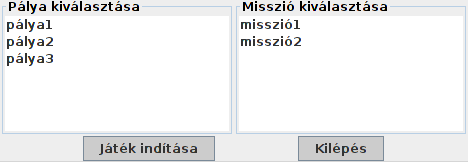
\includegraphics[width=10cm]{images/ch11/screenshot_menu.png}
\caption{A menü kinézete}
\label{fig:screenshot_menu}
\end{center}
\end{figure}

Értelemszerűen a bal oldali listában az elérhető pályák közül választhatja ki a felhasználó azt, amelyiken játszani szeretne, a jobb oldaliban pedig a kiválasztott pályához tartozó missziók közül azt, amelyiket el kívánja indítani.

Az alul látható gombok közül a ``Kilépés'' feliratú bezárja az alkalmazást, a ``Játék indítása'' feliratú pedig a fent kijelölt paraméterekkel elindítja a játékot. Ekkor az ablak átméreteződik, tartalma kicserélődik erre:

\begin{figure}[H]
\begin{center}
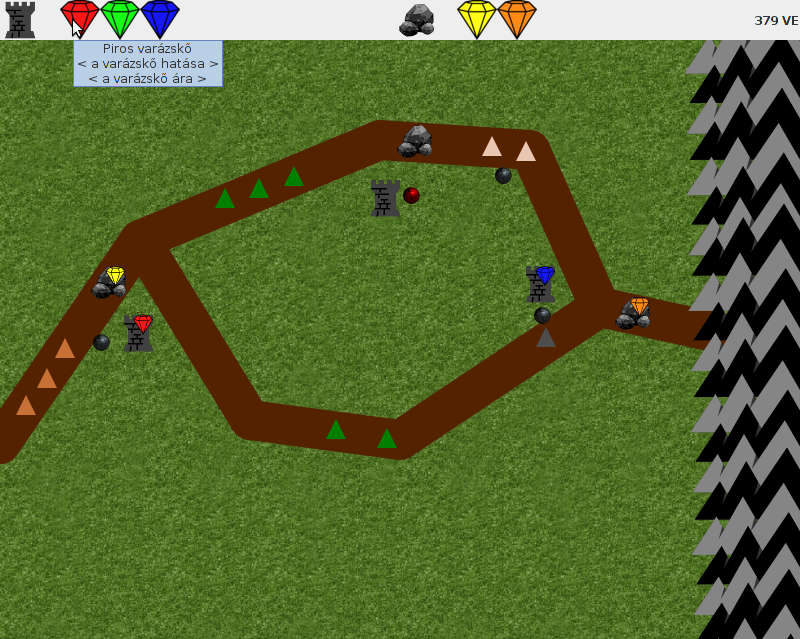
\includegraphics[width=14cm]{images/ch11/screenshot_game.png}
\caption{A játék képe}
\label{fig:screenshot_game}
\end{center}
\end{figure}

Az ablak felső részében a menüsáv, alatta pedig a játéktér foglal helyet.

A menüsávban lévő kis ikonok segítségével a következő funkciók érhetők el (balról jobbra haladva):

\begin{itemize}
\item Torony ikon: Először erre, majd a játéktéren egy megfelelő helyre (nem útra) kattintva egy torony építhető
\item Piros, zöld és kék varázskő ikonok: Először ezekre, majd a játéktéren egy toronyra kattintva egy torony erősíthető a kiválasztott varázskővel
\item Akadály ikon: Először erre, majd a játéktéren egy megfelelő helyre (útra) kattintva egy akadály építhető
\item Sárga és narancssárga varázskő ikonok: Először ezekre, majd a játéktéren egy akadályra kattintva egy akadály erősíthető a kiválasztott varázskővel
\end{itemize}

A menüsáv jobb szélén pedig a jelenleg rendelkezésre álló varázserőnket olvashatjuk le.\\
\\
Ahogyan a fenti ábrán is látszik, az egérmutatót a varázskő ikonokon tartva egy felugró eszköztipp ablakban megjelenik néhány sor szöveg, amely leírja a kiválasztott varázskő nevét, tulajdonságait, és varázserőben mért árát.\\
\\
A játéktér jeleníti meg a csata pillanatnyi állapotát. A barna vonalak az ellenség útvonalai, amelyeken az ablak jobb szélen látható Végzet Hegye felé tartanak.\\
\\
Az egyes ellenségeket különbözű színű háromszögek szimbolizálják. A sötétebb narancssárga embert, a halványrózsaszín hobbitot, a zöld tündét, a szürke pedig törpöt jelent.\\
\\
A tornyok magától értetődő ábrával jelennek meg, az akadályok az utakon pedig egy három szikladarabot ábrázoló kép formájában.\\
\\
Azon tornyok és akadályok képe fölött, amelyek már meg lettek erősítve varázskővel, a rajtuk lévő kő ikonja megjelenik a jobb felső sarokban.\\
\\
A tornyok által az ellenségekre kilőtt lövedékek a fekete, míg a különleges, kettévágó lövedékek a piros golyók.\\
\\
Az alkalmanként leszálló köd az egész játékteret beborító halvány, szürkés átfedés formájában fog megjelenni.\\
\\
Összefoglaló áttekintés a játéktér ikonjairól (nem méretarányosan):

\begin{figure}[ht]
\centering

\subfigure[Torony]{

\includegraphics[width=2cm]{images/ch11/icons/tower.png}
    \label{overview:tower}
}
\subfigure[Akadály]{

\includegraphics[width=2cm]{images/ch11/icons/obstacle.png}
    \label{overview:obstacle}
}
\subfigure[Varázskő]{

\includegraphics[width=2cm]{images/ch11/icons/blue_gem.png}
    \label{overview:gem}
}
\subfigure[Ellenség]{

\includegraphics[width=2cm]{images/ch11/icons/human.png}
    \label{overview:enemy}
}
\subfigure[Lövedék]{
\includegraphics[width=2cm]{images/ch11/icons/projectile.png}
    \label{overview:projectile}
}
\subfigure[Kettévágó lövedék]{
\includegraphics[width=2cm]{images/ch11/icons/splitter_projectile.png}
    \label{overview:splitter_projectile}
}
\caption{Áttekintés az ikonokról}
\label{fig:icon_overview}
\end{figure}

\newpage

\section{A grafikus rendszer architektúrája}
%\comment{A felület működésének elve, a grafikus rendszer architektúrája (struktúra diagramok). A struktúra diagramokon a prototípus azon és csak azon osztályainak is szerepelnie kell, amelyekhez a grafikus felületet létrehozó osztályok kapcsolódnak.}

\subsection{A felület működési elve}
A grafikus felületet MVC architektúrának megfelelően próbáltuk megtervezni. Minden képernyőn megjelenő objektumnak van egy grafikus párja, ami megvalósítja a \textbf{Drawable} interfészt. A \textbf{View} osztály ilyen objektumokat tárol, és minden kirajzolásnál meghívja ezen objektumok draw metódusát. \\
A megjelenítés push alapú. Ha a modelben történt valami változás (amit hívhatunk egy eseménynek), akkor értesíti a \textbf{View}-t, hogy valami esemény történt, úgy hogy meghívja az eseménynek megfelelő metódust. Kirajzolásnál minden grafikus objektum, lekérdezi a \textbf{Game}-ben lévő párjától az adatait, majd ez alapján kirajzolja magát. Esemény esetén nem történik kirajzolás. Kirajzolás csakis a drawAll() metódus hívásra történik, amit a Game adott időközönként meghív.\\
Az MVC megvalósítás alól kivételt képez a program indulása, amikor is egy egyszerű menü jelenik, amin el lehet indítani a játékot, ezt a \textbf{Menu} osztály végzi. Ez az osztály annyira egyszerű, hogy felesleges ebben is egy MVC-t megvalósítani.\\
A \textbf{Controller} osztály a program elején, a \textbf{Game} és \textbf{View} objektumok létrehozása után feliratkozik a neki megfelelő eseményekre. Ez után már fogadja is az eseményeket.\\
Tervezés során ügyletünk arra is, hogy könnyen bővíthető, cserélhető legyen a rendszer. A \textbf{View} és \textbf{Graphic} osztályokból való származtatással új GUI-t lehet készíteni, anélkül, hogy meglévő kódban kelljen (sokat) változtatni.

\subsection{A felület osztály-struktúrája}
%\comment{Osztálydiagram. Minden új osztály, és azon régiek, akik az újakhoz közvetlenül kapcsolódnak.}

\begin{figure}[H]
\begin{center}
\includegraphics[width=18cm]{images/ch11/very_final_uml_doge_diagram.png}
\caption{Grafikus felület osztálydigaramja}
\label{fig:Graphic_class_diag}
\end{center}
\end{figure}

\pagebreak
\section{A grafikus objektumok felsorolása}
%\comment{Az új osztályok felsorolása. Az régi osztályok közül azoknak a felsorolása, ahol változás volt. Ezek esetén csak a változásokat kell leírni.}

\subsection{Controller}
\begin{itemize}
\item Felelősség \newline
A játék futása közben a felhasználótól érkező eseményeket kezeli, és értesíti róluk a Game-et. Az egyes események kezelését továbbadja a benne lévő eseménykezelő osztályoknak.
\item Attribútumok
	\begin{itemize}
		\item - game: Game: A kontrollerhez tartozó Game onjektum.
		\item - view: View: A kontrollerhez tartozó View onjektum.
		\item - mapMouseEvent: MapMouseDelegate: Ez tárolja mi az elvégzendő művelet a térképen történő eseményeknél
		\item - activeButton: JButton: A jelenleg lenyomott gomb
	\end{itemize}
\item Metódusok
	\begin{itemize}
		\item - nullActiveButton(): Kitörli a kiválasztott gombot, beállítja a gombok kinézetét
	\end{itemize}
\end{itemize}

\subsection{+ Controller.MenuPanelMouseEvent}
\begin{itemize}
\item Felelősség \newline
A menüsávon való kattintás lekezelése.
\item Ősosztályok\newline
MouseAdapter
\item Metódusok
	\begin{itemize}
		\item + mousePressed(MouseEvent): Az egérkattintás eseménykezelője
	\end{itemize}
\end{itemize}

\subsection{+ Controller.MapMouseDelegate <<interface>>}
\begin{itemize}
\item Felelősség \newline
Egy interfész a térkép események kezelésére.
\item Metódusok
	\begin{itemize}
		\item + MapClicked(MouseEvent): Az egérkattintás eseménykezelője
		\item + MapMoved(MouseEvent): Az egérmozgatás eseménykezelője
	\end{itemize}
\end{itemize}

\subsection{Drawable}
\begin{itemize}
\item Felelősség \newline
Közös alapot biztosít a játékban az összes kirajzolható objektumnak.
\item Interfészek
\begin{itemize}
	\item Comparable<Drawable>: A kirajzolási sorrend megállapítása miatt van erre szükség.
\end{itemize}
\item Attribútumok
	\begin{itemize}
		\item \# img: Image: A kirajzolandó objektum képe.
		\item \# z\_index: int: A kirajzolandó objektum mélységi elhelyezkedése.
	\end{itemize}
\item Metódusok
	\begin{itemize}
		\item + \textit{draw(Graphics)}: Kirajzolja az objektumot.
		\item + compareTo(Drawable): int: Z-index szerint hasonlít össze két Drawable-t.
		\item + \underline{drawRangeCircle}(Graphics2D, Color, int x, int y, int radius): Egy kört rajzol ki az adott koordináták köré, a tornyok és akadályok hatótávolságának jelzésére van.
	\end{itemize}
\end{itemize}

\subsection{Game}
\begin{itemize}
\item Attribútumok
	\begin{itemize}
		\item - view: View: Egy referencia a grafikus megjelenítést végző osztályra.
	\end{itemize}
\end{itemize}

\subsection{GraphicEnemy}
\begin{itemize}
\item Felelősség \newline
Egy ellenség kirajzolása.
\item Ősosztályok\newline
Drawable
\item Attribútumok
	\begin{itemize}
		\item \# enemy: Enemy: A kirajzolandó ellenség.
	\end{itemize}
\item Metódusok
	\begin{itemize}
		\item + draw(Graphics): Kirajzolja az ellenséget.
		\item + equals(Object): boolean: Megadja, hogy két Graphic objektum egyenlő-e (ugyanazt a játékbeli objektumot reprezentálja).
	\end{itemize}
\end{itemize}

\subsection{GraphicFog}
\begin{itemize}
\item Felelősség \newline
A köd kirajzolása.
\item Ősosztályok\newline
Drawable
\item Metódusok
	\begin{itemize}
		\item + draw(Graphics): Kirajzolja a ködöt.
	\end{itemize}
\end{itemize}

\subsection{GraphicGem}
\begin{itemize}
\item Felelősség \newline
Egy varázskő kirajzolása lerakás közben.
\item Ősosztályok \newline
Drawable
\item Attribútumok
	\begin{itemize}
		\item \# pos: Vector: A varázskő jelenlegi helye.
	\end{itemize}
\item Metódusok
	\begin{itemize}
		\item + draw(Graphics): Kirajzolja a varázskövet.
		\item + getPosition(): Vector: Visszaadja a varázskő helyét.
	\end{itemize}
\end{itemize}

\subsection{GraphicMap}
\begin{itemize}
\item Felelősség \newline
A pálya kirajzolása.
\item Ősosztályok\newline
Drawable
\item Attribútumok
	\begin{itemize}
		\item \# map: Map: A kirajzolandó pálya.
		\item \# mountains: Image: A pálya jobb oldalán lévő hegyek képe.
	\end{itemize}
\item Metódusok
	\begin{itemize}
		\item + draw(Graphics): Kirajzolja a pályát.
		\item + equals(Object): boolean: Megadja, hogy két Graphic objektum egyenlő-e (ugyanazt a játékbeli objektumot reprezentálja).
	\end{itemize}
\end{itemize}

\subsection{GraphicObstacle}
\begin{itemize}
\item Felelősség \newline
Egy akadály kirajzolása.
\item Ősosztályok \newline
Drawable
\item Attribútumok
	\begin{itemize}
		\item \# obstacle: Obstacle: A kirajzolandó akadály.
		\item \# gemImage: Image: Az akadályra rakott varázskő képe.
	\end{itemize}
\item Metódusok
	\begin{itemize}
		\item + draw(Graphics): Kirajzolja az akadályt.
		\item + equals(Object): boolean: Megadja, hogy két Graphic objektum egyenlő-e (ugyanazt a játékbeli objektumot reprezentálja).
		\item + setGem(): Frissíti a kirajzolandó varázskő képét.
	\end{itemize}
\end{itemize}

\subsection{GraphicProjectile}
\begin{itemize}
\item Felelősség \newline
Egy lövedék kirajzolása.
\item Ősosztályok\newline
Drawable
\item Attribútumok
	\begin{itemize}
		\item \# projectile: Projectile: A kirajzolandó lövedék.
	\end{itemize}
\item Metódusok
	\begin{itemize}
		\item + draw(Graphics): Kirajzolja a lövedéket.
		\item + equals(Object): boolean: Megadja, hogy két Graphic objektum egyenlő-e (ugyanazt a játékbeli objektumot reprezentálja).
	\end{itemize}
\end{itemize}

\subsection{GraphicTower}
\begin{itemize}
\item Felelősség \newline
Egy torony kirajzolása.
\item Ősosztályok\newline
Drawable
\item Attribútumok
	\begin{itemize}
		\item \# tower: Tower: A kirajzolandó torony.
		\item \# gemImage: Image: A toronyra rakott varázskő képe.
	\end{itemize}
\item Metódusok
	\begin{itemize}
		\item + draw(Graphics): Kirajzolja a tornyot.
		\item + equals(Object): boolean: Megadja, hogy két Graphic objektum egyenlő-e (ugyanazt a játékbeli objektumot reprezentálja).
		\item + setGem(): Frissíti a kirajzolandó varázskő képét.
	\end{itemize}
\end{itemize}


\subsection{Menu}
\begin{itemize}
\item Felelősség \newline
A játék főmenüjét valósítja meg, amivel új játékot lehet indítani, ezen belül kiválasztani a pályát és a missziót.
\item Attribútumok
	\begin{itemize}
		\item \# panel: JPanel: A menü kirajzolásához használt JPanel.
	\end{itemize}
\item Metódusok
	\begin{itemize}
		\item + exit(): Bezárja a játék ablakait, és kilép a programból.
		\item + newGame(): Új játék indítását kezdeményezi.
		\item + run(): Elindítja a menü futását.
	\end{itemize}
\end{itemize}

\subsection{MouseEventHandler}
\begin{itemize}
\item Felelősség  \newline
Az egérkattintás eseményeket kezeli le.
\item Interfészek
\begin{itemize}
	\item MouseListener
\end{itemize}
\item Metódusok
	\begin{itemize}
		\item + MouseClicked(MouseEvent): Egérkattintáskor hívódik meg, kezeli az eseményt. Az egérkattintás pozíciójától függően meghívja a megfelelő metódust a Game-ben.
	\end{itemize}
\end{itemize}

\subsection{View}
\begin{itemize}
\item Felelősség \newline
A játék kirajzolása, azaz a Game osztály állapotának megjelenítésa a képernyőn.
\item Attribútumok
	\begin{itemize}
		\item - panel: JPanel: A játék kirajzolásához használt JPanel
		\item - drawables: List<Drawable>: A játékban kirajzolandó dolgok (ellenségek, tornyok, stb.) listája rendezve, hogy jó sorrenben legyen az objektumok kirajzolva.
		\item - mapPanel: JPanel: A játéknak a játékterét (pálya, ellenségek, tornyok, stb.) megjelenítő JPanel.
		\item - magicPanel: JPanel: A játék ezköztárát megjelenítő JPanel.
		\item - placing: Drawable: Azt az objektumot tárolja, ami épp lerakás alatt van, így ekkor is meg lehet jeleníteni.
	\end{itemize}
\item Metódusok
	\begin{itemize}
		\item + addDrawable(Drawable): Berak egy Drawable-t a kirajzolandó objektumok listájába.
		\item + drawAll(): Kirajzolja a játék jelenlegi állását.
		\item + enemyAdded(Enemy): A Game hívja meg amikor új ellenség kerül a pályára, frissíti a View adatstruktúráit.
		\item + enemyDied(Enemy): A Game hívja meg amikor meghal egy ellenség, frissíti a View adatstruktúráit.
		\item + gameLost(): Kirajzolja a vesztes játék végi üzenetet.
		\item + gameWon(): Kirajzolja a nyertes játék végi üzenetet.
		\item + getPanel(): Visszaadja a ``panel'' tagváltozót.
		\item + magicChange(int): Megváltoztatja a kiírt varázserő értéket a paraméterként kapottra.
		\item + obstacleAdded(Obstacle): A Game hívja meg amikor új akadály kerül a pályára, frissíti a View adatstruktúráit.
		\item + obstacleEnchanted(Obstacle): Frissíti egy meglévő akadály aktív varázskövét.
		\item - setButtonLook(JButton, ImageIcon): Beállítja egy JButton kinézetét.
		\item + setPlacing(Drawable): Beállítja az éppen lerakás alatt álló objektumot.
		\item + towerAdded(Tower): A Game hívja meg amikor új torony kerül a pályára, frissíti a View adatstruktúráit.
		\item + towerEnchanted(Tower): Frissíti egy meglévő torony aktív varázskövét.
		\item + projectileAdded(Projectile): A Game hívja meg amikor új lövedék kerül a pályára, frissíti a View adatstruktúráit.
		\item + projectileExploded(Projectile): A Game hívja meg amikor egy lövedék megsemmisül, frissíti a View adatstruktúráit.
		\item - winLoseScreen(String, Image): Kirajzolja a játék végi üzenetet és képet (nyerés/vesztés).
	\end{itemize}
\end{itemize}

\subsection{Window}
\begin{itemize}
\item Felelősség \newline
A játék fő ablaka, ez jeleníti meg a menüt és aztán magát a játékot.
\item Ősosztályok\newline
JFrame
\item Attribútumok
	\begin{itemize}
		\item - menu: Menu: A játék menü objektumát tárolja.
		\item - game: Game: A játék Game objektumát tárolja.
	\end{itemize}
\item Metódusok
	\begin{itemize}
		\item + setGame(Game): Beállítja azt a Game objektumot, amit a kezelőfelület meg fog jeleníteni. A menü fogja meghívni a pálya- és misszióválasztás után.
	\end{itemize}
\end{itemize}

\section{Kapcsolat az alkalmazói rendszerrel}
%\comment{Szekvencia-diagramokon ábrázolni kell a grafikus rendszer működését. Konzisztens kell legyen az előző alfejezetekkel. Minden %metódus, ami ott szerepel, fel kell tűnjön valamelyik szekvenciában. Minden metódusnak, ami szekvenciában szerepel, szereplnie kell a %valamelyik osztálydiagramon.}

\begin{figure}[H]
\begin{center}
\includegraphics[width=18cm]{images/grafikaSeq/init.png}
\caption{Játék inicializálása.}
\label{fig:Graphic_initialize}
\end{center}
\end{figure}

\begin{figure}[H]
\begin{center}
\includegraphics[width=18cm]{images/grafikaSeq/mouseTower.png}
\caption{Egérkattintásra torony lerakása.}
\label{fig:Graphic_mouse_tower}
\end{center}
\end{figure}

\begin{figure}[H]
\begin{center}
\includegraphics[width=18cm]{images/grafikaSeq/mouseOb.png}
\caption{Egérkattintásra akadály lerakása.}
\label{fig:Graphic_mouse_obstacle}
\end{center}
\end{figure}

\begin{figure}[H]
\begin{center}
\includegraphics[width=18cm]{images/grafikaSeq/mouseEnch.png}
\caption{Egérkattintásra torony vagy akadály varázskővel felruházása.}
\label{fig:Graphic_mouse_enchant}
\end{center}
\end{figure}

\begin{figure}[H]
\begin{center}
\includegraphics[width=18cm]{images/grafikaSeq/step1.png}
\caption{Az egész játék kirajzolása.(Map része)}
\label{fig:Graphic_drawAll_Map}
\end{center}
\end{figure}

\begin{figure}[H]
\begin{center}
\includegraphics[width=18cm]{images/grafikaSeq/step2.png}
\caption{Az egész játék kirajzolása.(Tower része)}
\label{fig:Graphic_drawAll_Tower}
\end{center}
\end{figure}

\begin{figure}[H]
\begin{center}
\includegraphics[width=18cm]{images/grafikaSeq/step3.png}
\caption{Az egész játék kirajzolása.(Obstacle része)}
\label{fig:Graphic_drawAll_Obstacle}
\end{center}
\end{figure}

\begin{figure}[H]
\begin{center}
\includegraphics[width=18cm]{images/grafikaSeq/step4.png}
\caption{Az egész játék kirajzolása.(Enemy része)}
\label{fig:Graphic_drawAll_Enemy}
\end{center}
\end{figure}

\begin{figure}[H]
\begin{center}
\includegraphics[width=18cm]{images/grafikaSeq/step5.png}
\caption{Az egész játék kirajzolása.(Projectile része)}
\label{fig:Graphic_drawAll_Projectile}
\end{center}
\end{figure}

\begin{figure}[H]
\begin{center}
\includegraphics[width=18cm]{images/grafikaSeq/step6.png}
\caption{Az egész játék kirajzolása.(Fog része)}
\label{fig:Graphic_drawAll_Fog}
\end{center}
\end{figure}

\begin{figure}[H]
\begin{center}
\includegraphics[width=18cm]{images/grafikaSeq/proj_Enemy_del.png}
\caption{Ellenség és lövedék törlése.}
\label{fig:Graphic_enemy/projectile_del}
\end{center}
\end{figure}

%% Szglab4
% ===========================================================================
%
\pagebreak
\section{Napló}
\begin{naplo}

\bejegyzes
{2014.04.25.~14:00~}
{0,5 óra}
{Nusser\newline
Tallér\newline
Török}
{Értekezlet. Grafikus felület architektúrájának és alap grafikus osztályok működésének megbeszélése.}

\bejegyzes
{2014.04.26.~11:00~}
{0,5 óra}
{Tallér}
{Tevékenység: osztálydiagram 1. változatának elkészítése}

\bejegyzes
{2014.04.26.~12:00~}
{0,5 óra}
{Szabó\newline
Tallér\newline
Török}
{Értekezlet. Architektúra megvitatása.}

\bejegyzes
{2014.04.27.~16:00~}
{1 óra}
{Tallér}
{Tevékenység: osztálydiagram befejezése, hozzá tartozó dokumentáció megírása.}

\bejegyzes
{2014.04.27.~17:00~}
{2 óra}
{Szabó\newline
Tallér\newline
Török}
{Tevékenység: A grafikus felület elemeinek, kinézetének összeállítása.}

\bejegyzes
{2014.04.27.~20:00~}
{3 óra}
{Török}
{Tevékenység: A felhasználói felület megtervezése, dokumentálása.}

\bejegyzes
{2014.04.27.~22:00~} % Kezdet
{3,5 óra} % Időtartam
{Szabó} % Résztvevők
{Osztályleírások elkészítése.} % Leírás

\bejegyzes
{2014.04.27.~21:00~}
{3 óra}
{Nusser}
{Tevékenység: Szekvencia diagramok készítése.}

\bejegyzes
{2014.04.28.~9:00~}
{0,5 óra}
{Tallér}
{Tevékenység: Dokumentációban hibák javítása, végső ellenőrzés.}

\end{naplo}

%
\setcounter{chapter}{12}
% Szglab4
% ===========================================================================
%
\chapter{Grafikus felület specifikációja}

\thispagestyle{fancy}

\section{Fordítási és futtatási útmutató}
%\comment{A feltöltött program fordításával és futtatásával kapcsolatos útmutatás. Ennek tartalmaznia kell leltárszerűen az egyes fájlok pontos nevét, méretét byte-ban, keletkezési idejét, valamint azt, hogy a fájlban mi került megvalósításra.}

\subsection{Fájllista}

\begin{fajllista}


\fajl
{icons/background.png}
{323033 byte}
{2014.05.03~19:15~}
{A játéktér háttérképe.}

\fajl
{icons/blue\_gem.png}
{2298 byte}
{2014.05.03~17:48~}
{A kék varázskövek ikonja.}

\fajl
{icons/dwarf.png}
{304 byte}
{2014.05.04~19:06~}
{A törpök ikonja.}

\fajl
{icons/elf.png}
{308 byte}
{2014.05.04~19:06~}
{A tündék ikonja.}

\fajl
{icons/green\_gem.png}
{2311 byte}
{2014.05.03~17:48~}
{A zöld varázskövek ikonja.}

\fajl
{icons/hobbit.png}
{319 byte}
{2014.05.04~19:06~}
{A hobbitok ikonja.}

\fajl
{icons/human.png}
{312 byte}
{2014.05.04~19:06~}
{Az emberek ikonja.}

\fajl
{icons/LZF.png}
{52032 byte}
{2014.05.05~16:29~}
{A játék megnyerésekor megjelenő kép.}

\fajl
{icons/obstacle.png}
{2430 byte}
{2014.05.03~17:48~}
{Az akadályok ikonja.}

\fajl
{icons/orange\_gem.png}
{2526 byte}
{2014.05.03~17:48~}
{A narancssárga varázskövek ikonja.}

\fajl
{icons/projectile.png}
{1167 byte}
{2014.05.04~19:22~}
{A lövedékek ikonja.}

\fajl
{icons/red\_gem.png}
{2302 byte}
{2014.05.03~17:48~}
{A piros varázskövek ikonja.}

\fajl
{icons/saurontower.png}
{43961 byte}
{2014.05.03~19:15~}
{A Végzet Hegyét és Szauron tornyát ábrázoló kép.}

\fajl
{icons/splitter\_projectile.png}
{905 byte}
{2014.05.04~19:22~}
{A kettévágó lövedékek ikonja.}

\fajl
{icons/tower.png}
{989 byte}
{2014.05.03~17:48~}
{A tornyok ikonja.}

\fajl
{icons/yellow\_gem.png}
{2443 byte}
{2014.05.03~17:48~}
{A sárga varázskövek ikonja.}


\fajl
{maps/demo.map}
{1228 byte}
{2014.05.04~20:42~}
{A felületi terven is látható pályafájl.}

\fajl
{maps/test.map}
{267 byte}
{2014.05.04~03:54~}
{Egy minimális pályafájl.}


\fajl
{missions/demo\_advanced.mission}
{5401 byte}
{2014.05.10~15:00~}
{Egy összetettebb missziófájl.}

\fajl
{missions/demo\_attack.mission}
{1251 byte}
{2014.05.04~20:42~}
{Egy egyszerű missziófájl.}

\fajl
{missions/demo\_delay.mission}
{1250 byte}
{2014.05.05~01:19~}
{Egy egyszerű missziófájl, hosszabb felkészülési idővel.}

\fajl
{missions/test\_attack.mission}
{139 byte}
{2014.05.04~03:54~}
{Egy minimális missziófájl.}



\fajl
{src/Controller.java}
{5456 byte}
{2014.05.03~15:20~}
{Az MVC modell controller részét valósítja meg.}

\fajl
{src/Drawable.java}
{2322 byte}
{2014.05.03~18:07~}
{A kirajzolható objektumok közös ősosztálya.}

\fajl
{src/Enemy.java}
{3362 byte}
{2014.03.20~20:33~}
{Az ellenségeket megvalósító osztály.}

\fajl
{src/EnemyType.java}
{998 byte}
{2014.03.21~12:57~}
{Az ellenségtípusokat leíró osztály.}

\fajl
{src/Fog.java}
{640 byte}
{2014.04.21~18:25~}
{A ködöt működtető osztály.}

\fajl
{src/Game.java}
{10064 byte}
{2014.03.20~09:55~}
{A játék logikáját összefogó osztály.}

\fajl
{src/Gem.java}
{409 byte}
{2014.03.21~12:57~}
{A varázskövek közös ősosztálya.}

\fajl
{src/GemButton.java}
{289 byte}
{2014.05.03~16:09~}
{A gombok, amelyekkel varázskövet lehet rakni az épületekre.}

\fajl
{src/GraphicEnemy.java}
{1205 byte}
{2014.05.03~18:07~}
{Az ellenségek kirajzolásáért felelős osztály.}

\fajl
{src/GraphicFog.java}
{432 byte}
{2014.05.03~21:32~}
{A köd kirajzolásáért felelős osztály.}

\fajl
{src/GraphicGem.java}
{1101 byte}
{2014.05.05~20:48~}
{A varázskövek kirajzolásáért felelős osztály.}

\fajl
{src/GraphicMap.java}
{2098 byte}
{2014.05.03~19:14~}
{A pálya kirajzolásáért felelős osztály.}

\fajl
{src/GraphicObstacle.java}
{2290 byte}
{2014.05.03~18:16~}
{Az akadályok kirajzolásáért felelős osztály.}

\fajl
{src/GraphicProjectile.java}
{1016 byte}
{2014.05.03~18:07~}
{A lövedékek kirajzolásáért felelős osztály.}

\fajl
{src/GraphicTower.java}
{2401 byte}
{2014.05.03~18:16~}
{A tornyok kirajzolásáért felelős osztály.}

\fajl
{src/Main.java}
{2645 byte}
{2014.05.04~19:32~}
{Az alkalmazást elindító osztály.}

\fajl
{src/Map.java}
{3801 byte}
{2014.03.20~20:33~}
{Egy pályát megvalósító osztály.}

\fajl
{src/Menu.java}
{6174 byte}
{2014.05.04~03:53~}
{A játék indító menüjét megvalósító osztály.}

\fajl
{src/Mission.java}
{2354 byte}
{2014.03.20~20:33~}
{Egy küldetést leíró osztály.}

\fajl
{src/Obstacle.java}
{2206 byte}
{2014.03.21~12:57~}
{Az akadályokat megvalósító osztály.}

\fajl
{src/ObstacleGem.java}
{805 byte}
{2014.03.20~20:33~}
{Az akadályokra tehető varázskövek.}

\fajl
{src/Pair.java}
{209 byte}
{2014.04.21~13:10~}
{Párokat tároló generikus osztály.}

\fajl
{src/Projectile.java}
{1219 byte}
{2014.03.20~20:33~}
{Egy lövedék viselkedését megvalósító osztály.}

\fajl
{src/Resources.java}
{1949 byte}
{2014.05.05~21:58~}
{Az összes játékban használt képet eltároló osztály.}

\fajl
{src/Spawn.java}
{302 byte}
{2014.04.22~00:59~}
{Egy konkrét ellenség típusát és játékba lépésének idejét tárolja.}

\fajl
{src/SplitterProjectile.java}
{729 byte}
{2014.04.21~17:43~}
{A kettévágó lövedékeket megvalósító osztály.}

\fajl
{src/Tower.java}
{3646 byte}
{2014.03.20~20:33~}
{Egy tornyot megvalósító osztály.}

\fajl
{src/TowerGem.java}
{902 byte}
{2014.03.20~20:33~}
{A tornyokra rakható varázskövek.}

\fajl
{src/Vector.java}
{1397 byte}
{2014.03.20~20:33~}
{Egy koordináta pontot megvalósító osztály.}

\fajl
{src/View.java}
{10510 byte}
{2014.05.03~14:31~}
{Az MVC modell view része.}

\fajl
{src/Waypoint.java}
{2208 byte}
{2014.03.21~12:57~}
{Az utakat kijelölő pontokat magvalósító osztály.}

\fajl
{src/Window.java}
{795 byte}
{2014.05.04~03:53~}
{A grafikus ablakot kezelő osztály.}

\end{fajllista}

\subsection{Fordítás}
%\comment{A fenti listában szereplő forrásfájlokból milyen műveletekkel lehet a bináris, futtatható kódot előállítani. Az előállításhoz csak a 2. Követelmények c. dokumentumban leírt környezetet szabad előírni.}

A fordításhoz lépjünk be egy terminálban a projekt főkönyvtárába, majd adjuk ki a következő parancsot:
\lstset{escapeinside=`', xleftmargin=10pt, frame=single, basicstyle=\ttfamily\footnotesize, language=sh}
\begin{lstlisting}
javac -d . -encoding utf8 src/szoftlab4/*.java
\end{lstlisting}

\subsection{Futtatás}
%\comment{A futtatható kód elindításával kapcsolatos teendők leírása. Az indításhoz csak a 2. Követelmények c. dokumentumban leírt környezetet szabad előírni.}
A futtatáshoz pedig a fordítást követően:
\lstset{escapeinside=`', xleftmargin=10pt, frame=single, basicstyle=\ttfamily\footnotesize, language=sh}
\begin{lstlisting}
java szoftlab4.Main
\end{lstlisting}

A fenti parancs után szóközzel elválasztva fűzhetünk még tetszés szerint kétféle parancssori argumentumot.
Egyikkel bekapcsolhatjuk az élsimítást (antialiasingot) a kirajzolásnál, a másikkal pedig a másodpercenként kirajzolt képkockák számát jeleníttethetjük meg a grafikus ablak jobb felső sarkában. Szokás szerint mindkét paraméternek van egy hosszú és egy rövid nevű változata.\\

A megszokott jelölést követve tehát a lehetséges opciók:

\begin{lstlisting}
java szoftlab4.Main [--antialiasing|-aa] [--showfps|-f]
\end{lstlisting}

\newpage

\section{Értékelés}
%\comment{A projekt kezdete óta az értékelésig eltelt időben tagokra bontva, százalékban.}

\begin{ertekeles}
\tag{Nusser} % Tag neve
{22}        % Munka szazalekban
\tag{Szabó}
{27}
\tag{Tallér}
{29}
\tag{Török}
{22}
\end{ertekeles}


% Szglab4
% ===========================================================================
%
\section{Napló}

\begin{naplo}

\bejegyzes
{2014.05.01.~16:00~}
{1 óra}
{Tallér}
{Tevékenység: Game osztály átalakítása.}

\bejegyzes
{2014.05.03.~14:00~}
{2,5 óra}
{Tallér}
{Tevékenység: View és Controller osztály elkészítése.}

\bejegyzes
{2014.05.03.~18:00~}
{1,5 óra}
{Nusser}
{Tevékenység: A grafikus osztályok megvalósítása.}

\bejegyzes
{2014.05.03.~22:00~}
{1 óra}
{Tallér}
{Tevékenység: Hibák javítása, apró módosítások.}

\bejegyzes
{2014.05.03.~20:00~}
{1,5 óra}
{Tallér}
{Tevékenység: Javítások, felhasználó felület élesztése.}

\bejegyzes
{2014.05.04.~02:00~}
{2 óra}
{Török}
{Tevékenység: A Window és a Menu osztályok megvalósítása.}

\bejegyzes
{2014.05.04.~19:00~}
{4 óra}
{Török}
{Tevékenység: Egy pálya- és egy missziófájl elkészítése, valamint rengeteg apró javítás eszközölése a kódon.}

\bejegyzes
{2014.05.04.~20:00~}
{2 óra}
{Szabó}
{Tevékenység: A View osztály frissítésének megvalósítása, útkirajzolás implementálása; kisebb javítások/módosítások.}

\bejegyzes
{2014.05.04.~23:00~}
{0,5 óra}
{Nusser}
{Tevékenység: Apróbb javítások a kódon.}

\bejegyzes
{2014.05.05.~14:00~}
{2 óra}
{Tallér}
{Tevékenység: Javítások, felhasználó felület csiszolása, hibakeresés.}

\bejegyzes
{2014.05.05.~16:00~}
{1 óra}
{Nusser}
{Tevékenység: Hibák javítása, kisebb fejlesztések.}

\bejegyzes
{2014.05.05.~01:00~}
{1 óra}
{Török}
{Tevékenység: A grafikus felület fejlesztése, javítása.}


\bejegyzes
{2014.05.05.~19:00~}
{2,5 óra}
{Szabó}
{Tevékenység: Az éppen építésre/lerakásra váró tornyok/akadályok/varázskövek folyamatos kirajzolásának implementálása, a képek betöltésének átrendezése.}

\bejegyzes
{2014.05.06.~14:00~}
{0,5 óra}
{Tallér}
{Tevékenység: Javítások, felhasználó felület csiszolása, hibakeresés.}

\bejegyzes
{2014.05.10.~12:00~}
{1 óra}
{Tallér}
{Tevékenység: Kommentezés, kisebb javítások.}

\bejegyzes
{2014.05.11.~12:00~}
{4 óra}
{Szabó}
{Tevékenység: Mindenféle javítás, kommentezés.}

\bejegyzes
{2014.05.11.~17:00~}
{1 óra}
{Nusser}
{Tevékenység: Kommentek írása.}

\bejegyzes
{2014.05.11.~23:00~}
{4 óra}
{Török}
{Tevékenység: Kommentezés, a fejezet dokumentációjának megírása.}


\end{naplo}


%
%\setcounter{chapter}{13}
%% Szglab4
% ===========================================================================
%
\chapter{Összefoglalás}

\thispagestyle{fancy}

\section{Projekt összegzés}
%\comment{A projekt tapasztalatait összegző részben a csapatoknak a projektről kialakult véleményét várjuk. A megválaszolandók köre az alábbi. }

\begin{munka}
\munkaido{Nusser}{46}
\munkaido{Szabó}{54.5}
\munkaido{Tallér}{58.5}
\munkaido{Török}{46.5}
\osszesmunkaido{205.5}
\end{munka}

\begin{forrassor}
\munkaido{Szkeleton}{962}
\munkaido{Protó}{1686}
\munkaido{Grafikus}{2993}
\end{forrassor}


\subsection{Nusser Ádám véleménye}
\begin{itemize}
\item Mit tanultak a projektből konkrétan és általában?\newline
	Ahogy hallottam, az iparban nincs mindig idő (soha), hogy ilyen részletesen megtervezzünk és dokumentáljunk egy programot, így jó volt legalább egyszer végigmenni a lépésin. Ezzel kicsit betekintést nyertünk szerintem a szoftveresek világába, amiből sokat tanultunk. A módszert ismertük, de így, hogy a gyakorlatban is láttuk, sokat segített abban, hogy valóban értelmét lássuk az egésznek. Hasznos volt még megismerni különböző programokat és nyelveket (Github, LateX, ...) melyek a jövőben is hasznosak lehetnek.
\newline Talán csapatmunkával kapcsolatban tanultuk a legkevesebbet, mert jól programozik és szorgalmas a csapat, így az egyéni munka sokkal több volt mint a csapatmunka, és míg ez nálunk működött, nagyon rossz vége is lehetett volna.
\item Mi volt a legnehezebb és a legkönnyebb? \newline
	A programváz tervezése volt talán a legnehezebb, hiszen nagyon nehéz olyan architektúrát tervezni, mely majd minden változtatás, és minden hozzáadott dolgot túléljen, és működjön nagyobb változtatások nélkül. A csapatban való dolgozás sem lett volna egyszerű, ha a csapattársaim nem lennének ilyen kiváló szakemberek, mert sajnos sokszor egyéni munkával oldottunk meg olyan feladatokat, melyeket sokkal egyszerűbben meg tudtunk volna oldani, ha leülünk és részletesebben átgondoljuk, megbeszéljük (ez főleg a vége felé igaz).
\newline A legegyszerűbb rész az implementáció volt, hiszen hetek óta azt terveztük, és mire oda értünk hogy kódolni kéne, már kentük-vágtuk, hogy mit fogunk nagyjából írni.
\item Összhangban állt-e az idő és a pontszám az elvégzendő feladatokkal? \newline
	Nagyrészt igen. Volt egy-két rész, amit ha az ember előtte jól megírt akkor később alig volt vele munka és mégis sok pontot ért, de ez így jó.
\item Ha nem, akkor hol okozott ez nehézséget? \newline
	Nem okozott.
\item Milyen változtatási javaslatuk van? \newline
	Szerintem a tervezéskor van egy-két olyan feladat, mely nagyon kicsi módosításokkal már szerepelt korábban, és így érdemi munkát nem ad, csak megy vele az idő (tudom, hogy a RUP része, de akkor is kihagyható lenne). Másrészt viszont a tesztelésre jobban kitérhetnénk, és kicsit jobban specifikált teszt feladatot kaphatnánk, mert az nem kap véleményem szerint annyi odafigyelést mint amennyit érdemelne.
\item Milyen feladatot ajánlanának a projektre? \newline
	Esetleg felül-nézetes, Rouge-like RPG-t lehetne feladni még a jövőben, mert nem túl nehéz megírni egy olyat, de jól meg kell tervezni, hogy könnyen bővíthető legyen.
\end{itemize}

\subsection{Tallér Bátor véleménye}
\begin{itemize}
\item Mit tanultak a projektből konkrétan és általában? \newline
Csapatban dolgozni nehéz, de egyben rengeteg dolgot megkönnyít. Ha valakire nincs kiadva feladat akkor az a feladat nem lesz megcsinálva.
A sok tervezés és dokumentáció után már könnyű azt leprogramozni.
\item Mi volt a legnehezebb és a legkönnyebb? \newline
A legnehezebb része a tervezés volt, konkrétan azon belül az, amikor kitaláltunk valamit majd később rájöttünk, hogy ez valamilyen ok miatt mégse megfelelő, és ezért újra kellett tervezni egyes részeket.\\
Továbbá nehézséget okozott összehangolni a projektet és az időnket.
\item Összhangban állt-e az idő és a pontszám az elvégzendő feladatokkal? \newline
Nagyjából összhangban állt. A súlyozással viszont nem értek egyet, mert pont a prototípussal dolgoztunk a legkevesebbet, míg a szkeletonnál sokat terveztünk és a grafikusnál meg sokat kódoltunk.\\
\item Ha nem, akkor hol okozott ez nehézséget? \newline
Nem okozott nehézségeket.
\item Milyen változtatási javaslatuk van? \newline
A dokumentáció sablonokat, illetve a tesztelési dokumentációkat aktualizálni kéne. A tesztelősben konkrétan ott áll az xls tetején, hogy 2009/2010, továbbá olyan kérdések voltak benne, amik nem tartoztak az aktuális feladathoz.\\\\
Véleményem szerint egy agilis módszertan jobb lenne a RUP helyett. Néhányszor azt éreztem, hogy a dokumentáció egyes részei feleslegesek (pl. állapotdiagram).\\\\
Hercules fejlesztése. Az az oldal azon kívül, hogy feltöltsük a beadandókat semmire se jó. Legalább az elért pontszámainkat feltüntethetné.
\item Milyen feladatot ajánlanának a projektre? \newline
Konkrét feladat nem jut az eszembe, de az ideihez hasonló teljesen megfelel a célra, mert nem csak egy unalmas program készül a végén, hanem egy működő játék.

\end{itemize}


\subsection{Török Attila véleménye}
\begin{itemize}

\item Mit tanultak a projektből konkrétan és általában? \newline
Konkrétan a \LaTeX{} nyelv alapjait, valamint git használatát, és annak segítségével munka megosztását DVCS-en keresztül, ugyanis eddig is használtam már verziókezelő rendszert, de nem gitet, és csak egyedül. Általában pedig azt, hogy egy nagyobb szoftver megtervezése és lefejlesztése, dokumentálása vajon hogyan is történhet(ett), még ha ez a projekt talán - László Zoltán tanár úr szavaival élve - ``kutyaólépítés toronydaruval'' volt is.

\item Mi volt a legnehezebb és a legkönnyebb? \newline
A legnehezebbnek a temérdek dokumentáció és számtalan diagram legyártását tartottam egy még nem létező dologról. Valahogy jobban tetszenek az iteratív fejlesztési módszerek, amik használatakor legalább a dokumentációval együtt fejlődik a program, még ha nem is a végleges verziója, de egy működő, futó prototípusa annak, és nem ilyen lineáris a dokumentációtól a kód felé haladás. Főleg a korai szakaszban való túlzottan részletekbe bocsátkozás kényszerítése idegenkedett tőlem, ugyanis úgy vélem, hogy az utolsó függvényparaméterig lehetetlen úgy megtervezni egy szoftvert, még egy ilyen kicsit is, hogy az végül illeszkedjen az eleinte elképzeltekre. Ha pedig a realizálódás során úgyis változni fognak a részletek, akkor egyáltalán miért írnánk le róluk egy légből kapott elképzelést? Persze a gondos, de viszonylag nagy vonalakban dolgozó architektúrális tervezést én is elengedhetetlennek tartom már a kezdetektől fogva.
Legkönnyebb nekem maga a lényegi kódolás volt, ugyanis abban már van gyakorlatom, és szívesen is csinálom, mert akkor érzem csak úgy, mintha valami működőt teremtenék.

\item Összhangban állt-e az idő és a pontszám az elvégzendő feladatokkal? \newline
A tárgyon belül kiosztott pontokat nem követtem minden feladatrésznél egészen pontosan nyomon, ezért erre nem tudok megfontolt választ adni, de az egyes csapattagok részvételi aránya és lelkesedése hétről hétre erősen ingadozhat, ezért a teher tetszés szerint megosztható.

\item Milyen változtatási javaslatuk van? \newline
Irreális követelménynek tartom a 6-os verziójú Java használatát, ugyanis ez már nem letölthető a gyártó hivatalos honlapjáról, ilyen régi JDK-t pedig szinte lehetetlen bárhol máshol találni, és JRE-t is csak kétséges forrásokból sikerült. Arra való tekintettel pedig, hogy nemrégiben megjelent a 8-as verzió, nem tartanám kizártnak, hogy egy év múlva már a 7-es sem lesz egykönnyen beszerezhető a HSZK pincéjében féltve őrzött lyukkártyáktól különböző médiumról.
Apróbb kellemetlenség volt még számomra a rendszeres hétfő reggeli beadási határidő.

\item Milyen feladatot ajánlanának a projektre? \newline
Nagyszerű ötletnek tartanék egy síkbeli Minecraft-szerű, ``ásós-szerkesztős-építős'' játékot.

\item Egyéb észrevételek, kritikák

Egy kicsit neheztelem azt is (igaz, legjobb tudomásom szerint ez már nem az Önök hatásköre, ezért csak mint véleményt, és nem mint kritikát írom), hogy ezért az 50-60 óra tényleges munkáért mindössze két kredit jár, ami - a legkisebb túlzás nélkül - mindenféle mókás kötelezően választható tárgyakból egyetlen délután alatt megszerezhető, némi szerencsével akár 4-es, vagy jobb érdemjeggyel. Nem magát az abszolút mértéket tartom inkorrektnek, tehát nem az a kérdés, hogy 1 kredit épp 5 vagy 150 órányi munkát jelképez elméletben, hanem abban látom a problémát, hogy a tárgyak között hatalmas szórás van az egy kreditért elvégzendő munkában, holott a későbbiekben már teljesen egyformán van kezelve, attól függetlenül, hogy milyen tantárgyból származik. Pedig szerintem az vitathatatlan, hogy a két órányi előadásra beüléshez (esetleg az arról való ellógáshoz) szükséges erőfeszítés meg sem közelíti a két órányi szekvenciadiagram-rajzoláshoz kellőt.

\end{itemize}


\subsection{Szabó Antal véleménye}
\begin{itemize}

\item Mit tanultak a projektből konkrétan és általában? \newline
Jó csapatban dolgozni, mert ha vannak olyan dolgok, amiket valaki nem szeret csinálni, jó esetben akkor is szét lehet úgy osztani a munkát, hogy mindenkinek elviselhető legyen. \newline
Konkrétan a Git és a \LaTeX{} használatában szereztem sok tapasztalatot, ami később jól jöhet.

\item Mi volt a legnehezebb és a legkönnyebb? \newline
Az egyik legnehezebb a program véleményem szerint túl részletes előre megtervezése volt, bármilyen kód írása nélkül. Nagyvonalakban természetesen meg kell előre tervezni, de a túl részletes tervezés szerintem felesleges, mert később úgy is lesznek benne változások, módosítások, amik már csak kód írásakor derülnek ki. A másik (ezzel összefüggően) a töménytelen mennyiségű dokumentáció írása volt, amiben sokszor lényegében ugyanazt kellett többször leírni akár egy fejezeten belül, akár a fejezetek között. \newline
A legkönnyebb (illetve legkellemesebb) rész a kód megírása volt, mert azt szeretem csinálni.

\item Milyen változtatási javaslatuk van? \newline
A dokumentáció sablonok és az ellenőrzőlapok aktualizálása; a dokumentációban lehetne kevesebb redundáns rész, illetve kevesebb olyan, ahova lényegében rizsázni kell.

\item Milyen feladatot ajánlanának a projektre? \newline
Konkrét ötletem nincs, de valamilyen játék írása azért jó, mert nem egy unalmas dolgot kell elkészíteni, hanem egy érdekes, a végén játszható programunk lesz.

\end{itemize}

%
%\clearpage
%
% Függelék
%
%\appendix
\end{document}
%
% EOF
%
